%% abtex2-modelo-artigo.tex, v<VERSION> laurocesar
%% Copyright 2012-<COPYRIGHT_YEAR> by abnTeX2 group at http://www.abntex.net.br/ 
%%
%% This work may be distributed and/or modified under the
%% conditions of the LaTeX Project Public License, either version 1.3
%% of this license or (at your option) any later version.
%% The latest version of this license is in
%%   http://www.latex-project.org/lppl.txt
%% and version 1.3 or later is part of all distributions of LaTeX
%% version 2005/12/01 or later.
%%
%% This work has the LPPL maintenance status `maintained'.
%% 
%% The Current Maintainer of this work is the abnTeX2 team, led
%% by Lauro César Araujo. Further information are available on 
%% http://www.abntex.net.br/
%%
%% This work consists of the files abntex2-modelo-artigo.tex and
%% abntex2-modelo-references.bib
%%

% ------------------------------------------------------------------------
% ------------------------------------------------------------------------
% abnTeX2: Modelo de Artigo Acadêmico em conformidade com
% ABNT NBR 6022:2018: Informação e documentação - Artigo em publicação 
% periódica científica - Apresentação
% ------------------------------------------------------------------------
% ------------------------------------------------------------------------

\documentclass[
	% -- opções da classe memoir --
	article,			% indica que é um artigo acadêmico
	12pt,				% tamanho da fonte
	oneside,			% para impressão apenas no recto. Oposto a twoside
	a4paper,			% tamanho do papel. 
	% -- opções da classe abntex2 --
	chapter=TITLE,		% títulos de capítulos convertidos em letras maiúsculas
	section=TITLE,		% títulos de seções convertidos em letras maiúsculas
	%subsection=TITLE,	% títulos de subseções convertidos em letras maiúsculas
	%subsubsection=TITLE % títulos de subsubseções convertidos em letras maiúsculas
	% -- opções do pacote babel --
	english,			% idioma adicional para hifenização
	brazil,				% o último idioma é o principal do documento 
	%sumario=abnt-6027-2012   % alternativa: sumario=tradicional
    sumario=tradicional
	]{abntex2}

% ---
% DADOS GERAIS DO TRABALHO PARA AS PÁGINAS INICIAIS
% ---

\newcommand{\MyInstitution}{Universidade Federal de Santa Maria}
\newcommand{\MyCenter}{Centro de Tecnologia}
\newcommand{\MyCourse}{Curso de Bacharelado em Ciência da Computação}
\newcommand{\MyDegree}{Bacharel em Ciência da Computação}
\newcommand{\MyTitle}{Avaliação qualitativa do pensamento computacional no ensino fundamental: um processo baseado em desafios Bebras e análise de estratégias de resolução com apoio de IA generativa}
%Da resolução à análise: um processo para avaliação qualitativa do pensamento computacional com desafios Bebras}
\newcommand{\MyForeignTitle}{Qualitative Assessment of Computational Thinking in Elementary Education: A Process Based on Bebras Challenges and the Analysis of Problem-Solving Strategies with Generative AI Support}
\newcommand{\MyAuthor}{Rafaela da Rosa Soares}
\newcommand{\MyFootnote}{Autor: Graduanda no \MyCourse~ pela \MyInstitution.}
\newcommand{\MyLocation}{Santa Maria, RS}

\newcommand{\MyDescriptionText}{Trabalho Final de Graduação apresentado ao \MyCourse~ da \MyInstitution~ (UFSM, RS), como requisito parcial para obtenção do grau de \textbf{\MyDegree}.}

\newcommand{\MyAdvisorName}{Andrea Schwertner Charão}
\newcommand{\MyAdvisorFootnote}{Orientadora: Professora do Departamento de Linguagens e Sistemas de Computação da \MyInstitution.}
\newcommand{\MyAdvisorTitle}{ORIENTADORA: Profa.}
\newcommand{\MyAdvisorCommitteeRole}{(Presidente/Orientadora)}
\newcommand{\MyFirstExaminer}{Silvia de Castro Bertagnolli (IFRS)}
\newcommand{\MySecondExaminer}{Leandro Krug Wives (UFRGS)}
\newcommand{\MyYear}{2026}
%\newcommand{\MyPresentationDate}{.. de ... de \MyYear}



% ---
% PACOTES
% ---

% ---
% Pacotes fundamentais 
% ---
%\usepackage{lmodern}			% Usa a fonte Latin Modern
\usepackage{times}              % Usa a fonte Times
\usepackage[T1]{fontenc}		% Selecao de codigos de fonte.
\usepackage[utf8]{inputenc}		% Codificacao do documento (conversão automática dos acentos)
\usepackage{indentfirst}		% Indenta o primeiro parágrafo de cada seção.
\usepackage{nomencl} 			% Lista de simbolos
\usepackage{color}				% Controle das cores
\usepackage{graphicx}			% Inclusão de gráficos
\usepackage{microtype} 			% para melhorias de justificação
\usepackage{setspace}
\usepackage{scalefnt}
\usepackage{amsfonts} % checkmarks
\usepackage{makecell}
\usepackage{float}

\usepackage{hyperref}
\usepackage{pdfpages}
\usepackage[utf8]{inputenc}
\usepackage{multicol}
\usepackage[justification=centering]{caption}

\usepackage{dirtree}
\usepackage{tabularx}
\usepackage{array}
\usepackage{caption}
\usepackage{placeins}
\usepackage{xltabular}
\usepackage{amsmath}
\usepackage{listings}

% \usepackage{trivfloat}
% \usepackage{chngcntr}
% \usepackage{float}

\usepackage{newfloat}
\usepackage{soul}
\usepackage{xcolor}

\usepackage{tikz}
\usetikzlibrary{arrows.meta, positioning}
% ---
	
% ---
% Pacotes de citações
% ---
\usepackage[brazilian,hyperpageref]{backref}	 % Paginas com as citações na bibl
\usepackage[alf,abnt-nbr10520=1988]{abntex2cite}

% \usepackage[alf]{abntex2cite}	% Citações padrão ABNT
%\usepackage{biblatex-abnt}
% Sobre atualização na norma de citações NBR 10520:2023:
% Ver https://groups.google.com/g/abntex2/c/yQ-AgdE9338?pli=1
% \usepackage[style=abnt]{biblatex}
% \renewcommand*{\mkbibnamefamily}[1]{#1}%
% ---


\usepackage{titling}

\usepackage{appendix}
\usepackage{listings}

\usepackage{setspace} % for \onehalfspacing and \singlespacing macros
\usepackage{xcolor}
\usepackage{colortbl}

\usepackage{textcomp}
\usepackage{etoolbox}

% --------------
% Configurações para code listing
% --------------
\definecolor{lightgray}{rgb}{.9,.9,.9}
\definecolor{darkgray}{rgb}{.4,.4,.4}
\definecolor{purple}{rgb}{0.65, 0.12, 0.82}
\definecolor{background}{rgb}{0.40, 0.42, 0.54}
\definecolor{keywords}{rgb}{0.65, 0.12, 0.82}


\let\quoteOld\quote
\let\endquoteOld\endquote


\renewenvironment{quote}{\small\quoteOld}{\endquoteOld}
%\renewenvironment{quote}{\quotefont\small\quoteOld}{\endquoteOld}


\renewcommand{\lstlistingname}{Bloco de código}
\lstdefinelanguage{JavaScript}{
  keywords={abstract, any, as, boolean, break, case, catch, class, console, const, continue, debugger, declare, default, delete, do, else, enum, export, 
    extends, false, finally, for, from, function, get, if, implements, import, in, 
    infer, instanceof, interface, keyof, let, module, namespace, never, new, null, 
    number, object, package, private, protected, public, readonly, require, return, 
    set, static, string, super, switch, symbol, this, throw, true, try, type, typeof, 
    undefined, unique, unknown, var, void, while, with, yield},
  keywordstyle=\color{blue}\bfseries,
  ndkeywords={class, export, boolean, throw, implements, import, this},
  ndkeywordstyle=\color{darkgray}\bfseries,
  identifierstyle=\color{black},
  sensitive=false,
  comment=[l]{//},
  morecomment=[s]{/*}{*/},
  commentstyle=\color{purple}\ttfamily,
  stringstyle=\color{red}\ttfamily,
  morestring=[b]',
  morestring=[b]"
}

\lstset{
   language=JavaScript,
   backgroundcolor=\color{lightgray},
   extendedchars=true,
   basicstyle=\footnotesize\ttfamily,
   showstringspaces=false,
   showspaces=false,
   numbers=none,  % left, right, none
   numberstyle=\footnotesize,
   numbersep=9pt,
   tabsize=2,
   breaklines=true,
   showtabs=false,
   captionpos=b
}

\lstdefinestyle{prompt}{
    basicstyle=\ttfamily\scriptsize,
    breaklines=true,
    columns=fullflexible,
    keepspaces=true,
    showstringspaces=false,
    extendedchars=true,
    inputencoding=utf8,
    literate=
        {á}{{\'a}}1
        {à}{{\`a}}1
        {ã}{{\~a}}1
        {â}{{\^a}}1
        {Á}{{\'A}}1
        {À}{{\`A}}1
        {Ã}{{\~A}}1
        {Â}{{\^A}}1
        {é}{{\'e}}1
        {ê}{{\^e}}1
        {É}{{\'E}}1
        {Ê}{{\^E}}1
        {í}{{\'i}}1
        {Í}{{\'I}}1
        {ó}{{\'o}}1
        {õ}{{\~o}}1
        {ô}{{\^o}}1
        {Ó}{{\'O}}1
        {Õ}{{\~O}}1
        {Ô}{{\^O}}1
        {ú}{{\'u}}1
        {Ú}{{\'U}}1
        {ç}{{\c{c}}}1
        {Ç}{{\c{C}}}1
}

%\setlength{\cftchapternumwidth}{20mm}
%\setlength{\cftsectionnumwidth}{20mm}
    
% ---
% Configurações do pacote backref
% Usado sem a opção hyperpageref de backref
\renewcommand{\backrefpagesname}{Citado na(s) página(s):~}
% Texto padrão antes do número das páginas
\renewcommand{\backref}{}
% Define os textos da citação
\renewcommand*{\backrefalt}[4]{
	\ifcase #1 %
		Nenhuma citação no texto.%
	\or
		Citado na página #2.%
	\else
		Citado #1 vezes nas páginas #2.%
	\fi}%
% ---




% --- Informações de dados para CAPA e FOLHA DE ROSTO ---
\titulo{\MyTitle}
\tituloestrangeiro{\MyForeignTitle}
\autor{\MyAuthor}
\local{\MyLocation}
\data{\MyYear}
\orientador{\MyAdvisor}
\instituicao{%
  \MyInstitution
  \par
  \MyCenter
  \par
  \MyCourse}
\tipotrabalho{Trabalho de Graduação}
% O preambulo deve conter o tipo do trabalho, o objetivo, 
% o nome da instituição e a área de concentração 
\preambulo{\MyDescriptionText}


% ---
% Configurações de aparência do PDF final

% alterando o aspecto da cor azul
\definecolor{blue}{RGB}{41,5,195}

% informações do PDF
\makeatletter
%\patchcmd{\@maketitle}{\LARGE}{\Huge}{\typeout{OK 1}}{\typeout{Failed 1}}

\hypersetup{
     	%pagebackref=true,
		pdftitle={\@title}, 
		pdfauthor={\@author},
    	pdfsubject={Modelo de artigo científico com abnTeX2},
	    pdfcreator={LaTeX with abnTeX2},
		pdfkeywords={abnt}{latex}{abntex}{abntex2}{artigo científico}, 
		colorlinks=true,       		% false: boxed links; true: colored links
    	linkcolor=blue,          	% color of internal links
    	citecolor=blue,        		% color of links to bibliography
    	filecolor=magenta,      		% color of file links
		urlcolor=blue,
		bookmarksdepth=4
}
\makeatother
% --- 



% ---
% compila o indice
% ---
\makeindex
% ---

% ---
% Altera as margens padrões
% ---
\setlrmarginsandblock{3cm}{3cm}{*}
\setulmarginsandblock{3cm}{3cm}{*}
\checkandfixthelayout
% ---




% --- 
% Espaçamentos entre linhas e parágrafos 
% --- 

% O tamanho do parágrafo é dado por:
\setlength{\parindent}{1.3cm}

% Controle do espaçamento entre um parágrafo e outro:
\setlength{\parskip}{0.2cm}  % tente também \onelineskip

% Espaçamento simples
\SingleSpacing




\renewcommand{\ABNTEXsectionfontsize}{\normalsize} 
\renewcommand{\ABNTEXsectionfont}{\normalfont\bfseries} 
\renewcommand{\ABNTEXsubsectionfontsize}{\normalsize} 
\renewcommand{\ABNTEXsubsectionfont}{\normalfont\bfseries} 


\renewcommand{\cftchapterfont}{\ABNTEXchapterfont\rmfamily}
\renewcommand{\cftsectionfont}{\ABNTEXsectionfont\rmfamily}
\renewcommand{\cftsubsectionfont}{\normalfont\rmfamily}
\renewcommand{\cftsubsubsectionfont}{\rmfamily}



\renewcommand{\maketitle}{%
  \begin{center}
  {\textbf{\MakeUppercase\thetitle}}\par
  {\MakeUppercase\theforeigntitle}\par\vspace{0.5cm}
  
  \textbf{\MyAuthor\footnote{\MyFootnote}, 
  \MyAdvisorName\footnote{\MyAdvisorFootnote}}\par
  \end{center}
}


\DeclareFloatingEnvironment[
  fileext=loq,
  listname=List of Quadros,
  name=Quadro,
  placement=htp,
]{quadro}

\captionsetup[quadro]{position=top}


% \trivfloat{quadro}
% \newcounter{quadro} % cria o contador
% \renewcommand{\thequadro}{\arabic{quadro}}
% \floatname{quadro}{Quadro}



% ----
% Início do documento
% ----
\begin{document}




%\renewcommand*{\l@section}{\@dottedtocline{1}{1em}{2em}}


%\renewcommand{\@pnumwidth}{1em}


% Seleciona o idioma do documento (conforme pacotes do babel)
%\selectlanguage{english}
\selectlanguage{brazil}

% Retira espaço extra obsoleto entre as frases.
%\frenchspacing 

% ----------------------------------------------------------
% ELEMENTOS PRÉ-TEXTUAIS
% ----------------------------------------------------------


%\setlength{\parskip}{0.0cm}
  \begin{center}
    %\singlespacing
    {\noindent\large{{\MakeUppercase{\MyInstitution}}}}\\%
    {\large{{\MakeUppercase{\MyCenter}}}}\\%
    {\large{{\MakeUppercase{{\MyCourse}}}}}\\%
    \vspace{8\baselineskip}
    {\Large{\scalefont{0.926}\theauthor}}\\
    \vspace{8\baselineskip}
    {\large\MakeUppercase{\textbf{\thetitle}}}\\
    \vspace{\fill}
    {\large{\MyLocation}}\\
    {\large{\MyYear}}
 \end{center}
%}

\newpage
     \begin{center}
        %\singlespacing
        \textbf{\noindent\theauthor}\\
        \vspace{6.0\baselineskip}
        \MakeUppercase{\textbf{\noindent{\thetitle}}}
        \vspace{4.0\baselineskip}
     \end{center}   
     
     \noindent\begin{flushright}
     \noindent\begin{minipage}{0.5\textwidth}
     %\singlespacing
     {\noindent \MyDescriptionText}
     % {\noindent Trabalho Final de Graduação apresentado ao \MyCourse~ da \MyInstitution~ (UFSM, RS), como requisito parcial para obtenção do grau de \textbf{\MyDegree}.}
     \end{minipage}
     \end{flushright}
            \vspace{7\baselineskip}
 
    \begin{center}
        %\singlespacing
        {{{\MyAdvisorTitle \MyAdvisorName}}}\\  
    \vspace{\fill}
        %{TG N. xxx\\ 
        {\MyLocation\\
        \MyYear}
    \end{center}

\newpage


% \includepdf{pdfs/aprovado_assinado_tcc.pdf}

% ----------------------------------------------------------
% Folha de assinaturas
% ----------------------------------------------------------



\setlength{\parskip}{0.0cm}

      \begin{center}
         \SingleSpacing
         \textbf{\noindent\theauthor}\\
         \vspace{6.0\baselineskip}
         \MakeUppercase{\textbf{\noindent\thetitle}}
         \vspace{4.0\baselineskip}
      \end{center}   
    
      \noindent\begin{flushright}
      \noindent\begin{minipage}{0.5\textwidth}
      \SingleSpacing
      {\noindent \MyDescriptionText}
 %      {\noindent Trabalho Final de Graduação apresentado ao
 % Curso de Bacharelado em Sistemas de Informação da Universidade Federal de Santa Maria (UFSM, RS), como requisito parcial para obtenção do grau de \textbf{\MyDegree.}}
      \end{minipage}
      \end{flushright}
    
      \SingleSpacing
      \vspace{0.25\baselineskip}
       \begin{center}

      \SingleSpacing
%      \textbf{Aprovado em \MyPresentationDate:}
      \vspace{2.0\baselineskip}




         \if@orientador
         \ifthenelse{\equal{\@orientadorpresidente}{P} \OR \equal{\@orientadorpresidente}{M}}
         \fi

        \vspace{1.0\baselineskip}
        \noindent\rule{0.5\textwidth}{1.pt}\\
        \noindent\textbf{\MyAdvisorName~ (UFSM)}\\
        \MyAdvisorCommitteeRole

        \vspace{1.0\baselineskip}
        \noindent\rule{0.5\textwidth}{1.pt}\\
        \noindent\textbf{\MyFirstExaminer}\\
        
        \vspace{1.0\baselineskip}
        \noindent\rule{0.5\textwidth}{1.pt}\\
        \noindent\textbf{\MySecondExaminer}\\
       
       
         \vspace{\fill}

         \MyLocation\\
         \MyYear
         \end{center}
         

\newpage

\begin{KeepFromToc}

\begin{center}
\end{center}

\newpage



\setlength{\parskip}{0.0cm}
      \vspace*{\fill}
      \begin{flushright}
      \begin{minipage}{0.45\textwidth}
      \textit{""}      
      \begin{flushright}\footnotesize{\textit{()}}\end{flushright}
      \end{minipage}
      \end{flushright}
      
\end{KeepFromToc}



\newpage

% página de titulo principal (obrigatório)
%\begin{titlingpage}
\maketitle
%\end{titlingpage}


% titulo em outro idioma (opcional)



% resumo em português
\begin{resumoumacoluna}
O Pensamento Computacional tem assumido papel crescente na Educação Básica, envolvendo habilidades relacionadas à resolução de problemas, como abstração, decomposição, reconhecimento de padrões, pensamento algorítmico e avaliação de soluções. Sua avaliação, entretanto, é complexa, especialmente quando se baseia predominantemente no resultado final das atividades, pois o acerto ou erro não revela, por si só, as estratégias utilizadas, as dificuldades encontradas, as tentativas realizadas ou as mudanças de raciocínio ocorridas durante a resolução. Este trabalho propõe uma abordagem qualitativa para investigar como estudantes do 8º ano do Ensino Fundamental mobilizam habilidades de Pensamento Computacional ao resolver problemas. Para isso, são utilizados desafios Bebras, por oferecerem tarefas estruturadas de resolução de problemas relacionadas à Computação e, em geral, independentes do domínio prévio de uma linguagem ou ambiente de programação. As atividades são acompanhadas de folhas-registro elaboradas para tornar observáveis aspectos do processo de resolução, como justificativas, representações, tentativas, formas de verificação e mudanças de estratégia, além de estimular a reflexão dos estudantes sobre o próprio raciocínio. A investigação é realizada em uma escola municipal de Santa Maria, Rio Grande do Sul, e combina uma etapa diagnóstica inicial com uma etapa reativa, na qual atividades posteriores são selecionadas a partir das evidências observadas nas aplicações anteriores. Como esse tipo de avaliação produz registros qualitativos mais ricos e numerosos do que respostas objetivas isoladas, o trabalho também investiga um fluxo computacional de apoio à digitalização, organização e análise dos dados, com uso de reconhecimento óptico de caracteres e inteligência artificial generativa, mantendo a conferência dos registros originais e a interpretação humana. Espera-se contribuir para a discussão sobre formas de avaliação do Pensamento Computacional que considerem o processo de resolução e para a construção de um processo reutilizável de apoio à análise qualitativa em contexto escolar.

%\vspace{\onelineskip}
 
 \noindent
 \textbf{Palavras-chave}: Pensamento Computacional; Bebras; Avaliação qualitativa; Estratégias de resolução; Inteligência artificial generativa.
 
\end{resumoumacoluna}


% resumo em inglês
\renewcommand{\resumoname}{Abstract}
\begin{resumoumacoluna}
\begin{otherlanguage*}{english}

Computational Thinking has assumed an increasingly important role in Basic Education, encompassing problem-solving skills such as abstraction, decomposition, pattern recognition, algorithmic thinking, and solution evaluation. Assessing these skills, however, is challenging, especially when evaluation relies primarily on the final outcome of an activity, since a correct or incorrect answer alone does not reveal the strategies used, the difficulties encountered, the attempts made, or changes in reasoning during problem solving. This study proposes a qualitative approach to investigate how 8th-grade students mobilize Computational Thinking skills while solving problems. Bebras challenges are used because they provide structured computing-related problem-solving tasks that are generally independent of prior knowledge of a programming language or environment. The activities are accompanied by recording sheets designed to make aspects of the problem-solving process observable, including justifications, representations, attempts, verification procedures, and changes in strategy, while also encouraging students to reflect on their own reasoning. The study is conducted at a municipal school in Santa Maria, Rio Grande do Sul, Brazil, and combines an initial diagnostic stage with a reactive stage, in which subsequent activities are selected based on evidence observed in previous applications. Because this type of assessment produces richer and more numerous qualitative records than isolated objective answers, the study also investigates a computational workflow to support data digitization and organization using optical character recognition and generative artificial intelligence, while retaining the original records for verification and human interpretation. The study aims to contribute to the discussion of Computational Thinking assessment approaches that consider the problem-solving process and to the development of a reusable workflow for supporting qualitative analysis in school contexts.

\noindent
\textbf{Keywords}: Computational Thinking; Bebras; Qualitative assessment; Problem-solving strategies; Generative artificial intelligence.

\end{otherlanguage*}
\end{resumoumacoluna}

% ]  				% FIM DE ARTIGO EM DUAS COLUNAS
% ---

% \begin{center}\smaller
% \textbf{Data de submissão e aprovação}: elemento obrigatório. Indicar dia, mês e ano

% \textbf{Identificação e disponibilidade}: elemento opcional. Pode ser indicado 
% o endereço eletrônico, DOI, suportes e outras informações relativas ao acesso.
% \end{center}
\newpage

\begin{KeepFromToc}
    \renewcommand\listfigurename{Lista de Figuras}
    \listoffigures
    \newpage

    % \listofquadro
    % \newpage
    %\listoftables
    %\newpage
        
    \tableofcontents
    \thispagestyle{empty}
    \newpage
\end{KeepFromToc}

% ----------------------------------------------------------
% ELEMENTOS TEXTUAIS
% ----------------------------------------------------------
\textual

% -------------------------------------------------------------------------------------
% Introdução
% -------------------------------------------------------------------------------------
\section{Introdução}
\label{sec:introducao}

A presença da Computação na Educação Básica envolve conhecimentos e práticas que vão além do domínio de ferramentas digitais ou da aprendizagem de linguagens de programação. Entre os conhecimentos associados à área, destaca-se o Pensamento Computacional, entendido como um conjunto de formas de organizar e resolver problemas de maneira metódica. No contexto educacional brasileiro, a Base Nacional Comum Curricular (BNCC) \cite{brasil2018} e as Normas sobre Computação na Educação Básica -- Complemento à BNCC \cite{cne2022} reconhecem o Pensamento Computacional como um eixo formativo relacionado, entre outros aspectos, à criação e análise de algoritmos, à identificação de padrões, à decomposição de problemas e à elaboração de representações que auxiliem na resolução de situações-problema.

A inserção da Computação na Educação Básica vem sendo ampliada por iniciativas institucionais recentes. Em 2022, a Resolução CNE/CEB nº 1 estabeleceu as Normas sobre Computação na Educação Básica -- Complemento à BNCC \cite{cne2022}. No ano seguinte, a Lei nº 14.533 instituiu a Política Nacional de Educação Digital \cite{brasil2023pned}, contemplando ações relacionadas à inclusão digital e à Educação Digital Escolar. Esse cenário amplia a necessidade de compreender como conhecimentos e habilidades de Computação se manifestam nas atividades realizadas pelos estudantes.

A avaliação do Pensamento Computacional, porém, apresenta desafios. Uma resposta correta, considerada isoladamente, informa pouco sobre a forma como o estudante organizou o problema, as estratégias que testou, as representações que utilizou ou os procedimentos empregados para verificar a solução. Uma resposta incorreta também pode conter elementos relevantes do processo, como tentativas de decomposição, identificação de relações, revisão de hipóteses ou construção de sequências. Em revisão sistemática da área, \citeonline{tang2020} identificaram diferentes instrumentos de avaliação, incluindo testes, avaliações de desempenho, análise de produções e questionários, mostrando que diferentes formas de coleta tornam visíveis dimensões distintas do Pensamento Computacional.

As atividades do Desafio Bebras oferecem um contexto adequado para investigar esses processos. O Bebras é uma iniciativa internacional voltada à promoção da Computação e do Pensamento Computacional na Educação Básica. Suas tarefas apresentam problemas curtos, contextualizados e, em geral, independentes de conhecimento prévio de programação. No Brasil, o regulamento do desafio associa as tarefas às habilidades de abstração, pensamento algorítmico, decomposição, avaliação e reconhecimento de padrões, admitindo que uma mesma questão possa mobilizar várias dessas habilidades \cite{bebras2026}. \citeonline{dejong2024}, ao analisarem qualitativamente a resolução de tarefas Bebras, observaram que as habilidades mobilizadas durante o processo nem sempre correspondem diretamente ao acerto da questão.

A partir dessas questões, este trabalho investiga como atividades Bebras, acompanhadas de registros sobre o processo de resolução, podem apoiar a identificação qualitativa da mobilização de habilidades de Pensamento Computacional por estudantes do 8º ano do Ensino Fundamental. O objetivo geral é analisar como esses estudantes mobilizam tais habilidades durante a resolução das atividades, considerando respostas, justificativas, representações, tentativas, formas de verificação e mudanças de estratégia registradas ao longo do processo.

A investigação surgiu no contexto de atividades desenvolvidas com uma turma de 8º ano da Escola Municipal de Ensino Fundamental Lívia Menna Barreto, em Santa Maria, Rio Grande do Sul, vinculadas ao projeto de extensão ``Conectando Saberes: Letramento Digital para Discentes em Instituições de Ensino'', da Universidade Federal de Santa Maria. A experiência com a turma motivou a busca por instrumentos capazes de registrar como os estudantes constroem suas respostas e quais dificuldades percebem durante a resolução. Os detalhes sobre participantes, organização dos encontros e critérios de seleção das atividades são apresentados na metodologia.

Para tornar esses processos observáveis, as tarefas Bebras são acompanhadas de folhas de registro que solicitam justificativas, representações, tentativas, procedimentos de verificação, dificuldades percebidas e eventuais mudanças de estratégia. Esses registros ampliam as evidências disponíveis para a análise e também favorecem momentos de reflexão dos estudantes sobre o próprio raciocínio. A reflexão sobre o processo é utilizada como fonte complementar de informação, sem constituir, neste estudo, uma avaliação independente de metacognição.

O aumento da quantidade e da diversidade de registros produzidos cria outro desafio: organizar de forma sistemática textos manuscritos, desenhos, sequências, rasuras e marcações sem perder o vínculo com as folhas originais. Por essa razão, o trabalho também investiga um processo computacional de apoio à digitalização, extração e estruturação dos dados, envolvendo reconhecimento óptico de caracteres e inteligência artificial generativa. Os recursos automatizados são empregados para organizar o material e facilitar sua localização e conferência, enquanto a interpretação das evidências permanece vinculada aos critérios definidos para a pesquisa e à leitura dos registros originais.

A contribuição do trabalho está na articulação de três elementos: desafios Bebras, instrumentos voltados ao registro do processo de resolução e um processo computacional de apoio à organização das evidências qualitativas. A proposta busca produzir um procedimento reutilizável que permita examinar, de forma rastreável, diferentes aspectos da resolução dos problemas e que possa ser refinado a partir da experiência obtida nas aplicações.

A relevância da pesquisa está relacionada à possibilidade de produzir informações úteis para além da correção da alternativa final. Para professores e para a escola participante, a identificação de dificuldades, estratégias recorrentes e formas de verificação pode apoiar o planejamento de atividades posteriores. No âmbito acadêmico, o estudo contribui para a discussão sobre avaliação qualitativa do Pensamento Computacional com tarefas Bebras e explora o uso de tecnologias atuais para apoiar a organização de registros detalhados produzidos em contexto escolar.

\subsection{Objetivo geral}

Analisar, de forma qualitativa, como estudantes do 8º ano mobilizam habilidades de Pensamento Computacional durante a resolução de atividades Bebras.

\subsection{Objetivos específicos}

\begin{itemize}
    \item Mapear habilidades de Pensamento Computacional relacionadas ao contexto do 8º ano do Ensino Fundamental;
    \item selecionar atividades Bebras que mobilizem as habilidades investigadas;
    \item definir um método de coleta que permita registrar estratégias e processos de resolução utilizados pelos estudantes;
    \item aplicar as atividades selecionadas em contexto escolar;
    \item analisar respostas, justificativas, representações e processos de resolução;
    \item identificar dificuldades, estratégias recorrentes e indícios de mobilização das habilidades observadas;
    \item desenvolver e experimentar um processo computacional de apoio à digitalização, extração, estruturação e organização dos registros produzidos pelos estudantes;
    \item analisar as possibilidades e limitações do uso de reconhecimento óptico de caracteres e inteligência artificial generativa como apoio à organização de dados qualitativos.

\end{itemize}

% -------------------------------------------------------------------------------------
% Fundamentação teórica
% -------------------------------------------------------------------------------------

\section{Fundamentação teórica}
\label{sec:fundamentacao}

\subsection{Pensamento Computacional e suas habilidades}

O Pensamento Computacional refere-se a formas de raciocínio oriundas da Ciência da Computação que podem ser utilizadas na formulação e resolução de problemas. \citeonline{wing2006} relaciona o conceito à formulação de problemas e à construção de soluções que possam ser representadas e executadas de maneira sistemática. Apesar da ampla utilização do termo, não existe uma definição única. Revisões como as de \citeonline{grover2013} e \citeonline{shute2017} mostram que diferentes referenciais enfatizam conjuntos distintos de conceitos, práticas e habilidades.

Entre esses referenciais, \citeonline{brennan2012} organizam o Pensamento Computacional em conceitos computacionais, práticas computacionais e perspectivas computacionais. As práticas incluem, entre outras ações, testar, depurar e abstrair, destacando a importância dos procedimentos utilizados durante a construção de uma solução.

No contexto brasileiro, a Base Nacional Comum Curricular e as Normas sobre Computação na Educação Básica incorporam conhecimentos relacionados ao Pensamento Computacional à formação dos estudantes \cite{brasil2018,cne2022}. O complemento de Computação à BNCC organiza as aprendizagens da área nos eixos Pensamento Computacional, Mundo Digital e Cultura Digital, sendo o primeiro diretamente relacionado à formulação e resolução de problemas, algoritmos, decomposição, modelagem e representação de soluções.

Essas habilidades também podem ser trabalhadas em atividades desplugadas. \citeonline{brackmann2017} demonstra a possibilidade de explorar conceitos associados ao Pensamento Computacional sem depender do uso de computadores ou de linguagens de programação.

Neste trabalho, são consideradas cinco habilidades como referência para a seleção e análise das atividades: pensamento algorítmico, decomposição, abstração, avaliação e reconhecimento de padrões \cite{brackmann2017,bebras2026}. A classificação adotada acompanha as categorias utilizadas pelo Bebras Brasil e admite que diferentes habilidades possam aparecer simultaneamente em uma mesma estratégia de resolução.

O pensamento algorítmico está relacionado à organização de uma solução em uma sequência de passos ou regras. A decomposição envolve dividir um problema em partes menores para facilitar sua análise. A abstração corresponde à seleção das informações relevantes e à construção de representações que reduzam detalhes desnecessários. A avaliação envolve examinar uma solução, comparar possibilidades e identificar inconsistências, podendo incluir ações de depuração. O reconhecimento de padrões envolve identificar regularidades ou relações que possam ser utilizadas na resolução de um problema.

\subsection{Avaliação do Pensamento Computacional}

A diversidade de definições de Pensamento Computacional também se reflete nas formas utilizadas para avaliá-lo. \citeonline{tang2020}, em revisão sistemática de estudos empíricos, identificaram instrumentos como testes, avaliações de desempenho, portfólios, questionários e análise de produções. Essa variedade indica que diferentes instrumentos podem tornar visíveis aspectos distintos do construto.

Estudos que investigam o processo de resolução têm recorrido à combinação de diferentes fontes de evidência. \citeonline{brennan2012}, por exemplo, utilizaram análise de projetos, entrevistas baseadas em artefatos e situações de projeto para investigar o desenvolvimento do Pensamento Computacional. \citeonline{grover2015} também defendem a utilização de sistemas de avaliação que articulem respostas, produções, observações e explicações dos estudantes.

Essa perspectiva é especialmente relevante em tarefas de resolução de problemas. A resposta final informa o resultado alcançado, mas não permite reconstruir, por si só, as estratégias utilizadas durante o percurso. Em estudo com tarefas Bebras, \citeonline{dejong2024} observaram que as habilidades mobilizadas pelos participantes durante a resolução nem sempre correspondiam diretamente ao acerto da questão.

A utilização da pontuação do Bebras como medida de Pensamento Computacional também exige cautela. \citeonline{araujo2017} encontraram correlação moderada entre o desempenho em tarefas simuladas do Bebras e as notas de estudantes em disciplinas introdutórias de programação. Posteriormente, \citeonline{araujo2019} verificaram que a estrutura teórica de cinco habilidades inicialmente considerada não encontrou suporte estatístico direto nos dados analisados.

Neste trabalho, a avaliação possui caráter qualitativo e diagnóstico. A análise procura identificar evidências das habilidades durante a resolução das tarefas, considerando respostas, justificativas, representações, tentativas, procedimentos de verificação e mudanças de estratégia. As categorias utilizadas descrevem aquilo que pode ser sustentado pelos registros produzidos em cada atividade, preservando o limite entre ausência de evidência e ausência da habilidade.

\subsection{Processos de resolução e reflexão sobre o próprio raciocínio}

Durante a resolução de um problema, o estudante pode interpretar o enunciado, selecionar informações, construir representações, testar alternativas, revisar hipóteses e verificar a solução. Parte dessas ações pode ser registrada durante a atividade e utilizada como fonte de evidência sobre o processo empregado.

Métodos voltados à observação do processo buscam tornar parte desse percurso acessível à análise. \citeonline{ericsson1993} discutem o uso de relatos verbais para investigar processos cognitivos durante a execução de tarefas. No contexto do Pensamento Computacional, \citeonline{dejong2024} empregaram o método \textit{think-aloud} para acompanhar participantes enquanto resolviam tarefas Bebras.

A presente pesquisa utiliza folhas de registro em vez de um protocolo contínuo de \textit{think-aloud}. Os estudantes podem explicar como chegaram à resposta, registrar etapas, indicar possibilidades consideradas e utilizar desenhos, setas, tabelas ou sequências. Esses elementos são interpretados em conjunto com a tarefa, a resposta final e os demais registros produzidos durante a aplicação, constituindo evidências parciais do processo de resolução.

\subsection{Desafios Bebras e Pensamento Computacional}

O Bebras é uma iniciativa internacional voltada à promoção da Informática e do Pensamento Computacional na Educação Básica por meio de desafios de resolução de problemas. As tarefas são curtas,
contextualizadas e destinadas a diferentes faixas etárias, geralmente sem exigir conhecimento prévio de uma linguagem de programação \cite{dagiene2016}.

No Bebras Brasil, as atividades são associadas às habilidades de abstração, pensamento algorítmico, decomposição, avaliação e reconhecimento de padrões. Uma mesma tarefa pode envolver diferentes
habilidades, dependendo das características do problema e da estratégia utilizada pelo estudante \cite{bebras2026}. Por essa razão, a classificação das tarefas é utilizada nesta pesquisa como referência para sua seleção e para a definição inicial das evidências a serem observadas.

Estudos anteriores indicam diferentes possibilidades de utilização do Bebras em processos de avaliação. \citeonline{dejong2024} analisaram qualitativamente as habilidades mobilizadas durante a resolução das tarefas. No Brasil, \citeonline{araujo2017} investigaram sua utilização como instrumento de avaliação em cursos introdutórios de programação, enquanto \citeonline{alves2025} empregaram tarefas Bebras em avaliações com estudantes do 8º ano. \citeonline{nipo2026} utilizaram o desafio como instrumento de comparação na avaliação de um jogo digital voltado ao Pensamento Computacional.

Neste trabalho, as tarefas Bebras são utilizadas como situações-problema para observar estratégias de resolução. Cada atividade é acompanhada por uma folha de registro elaborada para coletar justificativas, representações, tentativas, procedimentos de verificação e mudanças de estratégia. A análise considera esses elementos em conjunto com a resposta apresentada pelo estudante.

\subsection{Inteligência artificial generativa no apoio à análise de dados qualitativos}
\label{subsec:ia-generativa}

A opção por registrar o processo de resolução amplia a quantidade e a diversidade dos dados produzidos pela pesquisa. Em vez de respostas objetivas isoladas, passam a fazer parte do conjunto de dados textos manuscritos, sequências, desenhos, rasuras, justificativas e outras representações. A organização manual desse material pode demandar tempo significativo, principalmente quando as atividades são aplicadas repetidamente ao longo de um período letivo.

Tecnologias de reconhecimento óptico de caracteres (OCR) podem apoiar a transformação de documentos digitalizados em conteúdo textual, reduzindo parte do trabalho de transcrição. Entretanto, a extração do texto não equivale à sua interpretação. Registros qualitativos podem apresentar relações entre elementos, símbolos, correções e estruturas que exigem organização posterior antes de serem utilizados na análise.

É importante distinguir, nesse contexto, o reconhecimento de caracteres da interpretação realizada por modelos generativos. O OCR tem como finalidade principal converter elementos presentes em um documento digitalizado em uma representação textual. Já um modelo generativo pode receber esse conteúdo e transformá-lo segundo uma instrução, por exemplo identificando campos, reorganizando respostas ou produzindo uma estrutura padronizada. Em sistemas multimodais, o próprio modelo também pode processar imagens, mas isso não elimina a necessidade de distinguir erros de leitura do documento de erros produzidos durante a interpretação ou estruturação das informações. Essa separação é relevante para a rastreabilidade do processo e para a identificação da etapa em que uma informação pode ter sido alterada.

Modelos de inteligência artificial generativa, especialmente modelos de linguagem de grande porte, têm sido investigados como ferramentas de apoio ao processamento de dados qualitativos. \citeonline{depaoli2024}, ao experimentar um modelo de linguagem na análise temática de entrevistas, mostra que esses sistemas podem auxiliar na identificação e organização de informações, ao mesmo tempo em que ressalta que a análise qualitativa envolve interpretação e não pode ser reduzida à geração automática de categorias. \citeonline{parfenova2024} também discutem o uso de modelos de linguagem para automatizar etapas de codificação qualitativa e apontam a necessidade de investigar seus limites e sua relação com a análise realizada por pesquisadores humanos.

Um aspecto relevante é que as respostas produzidas por modelos generativos dependem das instruções fornecidas. O prompt delimita a tarefa solicitada, os critérios considerados e o formato esperado da saída. Assim, quando esses modelos são empregados como parte de um processo de pesquisa, a descrição das instruções utilizadas e do formato dos resultados torna-se importante para permitir rastreabilidade e reprodução do procedimento.

Além disso, modelos generativos podem produzir interpretações incorretas, omitir informações ou apresentar resultados diferentes diante de pequenas mudanças na entrada e nas instruções. Em dados manuscritos, esses problemas podem ser precedidos ainda por erros de reconhecimento do documento original. Por esse motivo, a utilização dessas tecnologias exige mecanismos de conferência que mantenham vínculo entre a informação estruturada automaticamente e o registro produzido pelo participante.

No presente trabalho, a inteligência artificial é investigada como apoio à extração, estruturação e organização dos registros, e não como substituta da análise qualitativa realizada pelo pesquisador. O fluxo computacional em desenvolvimento combina reconhecimento óptico de caracteres com uma etapa de interpretação estruturada por modelo generativo, produzindo informações que podem ser organizadas para análise posterior. A saída automática permanece sujeita à conferência em relação às folhas originais.

Essa abordagem busca explorar uma contribuição computacional do trabalho: construir um processo reutilizável capaz de reduzir tarefas manuais de organização sem retirar do pesquisador a responsabilidade pela interpretação. Na metodologia serão detalhados os dados fornecidos ao sistema, as instruções utilizadas, o formato de saída, os procedimentos de conferência e os cuidados adotados no tratamento dos registros dos estudantes.

\section{Metodologia}

A pesquisa adota abordagem qualitativa, de caráter exploratório e
descritivo, organizada como estudo de caso em contexto escolar
\cite{andre2013}. A metodologia combina produções individuais,
registros de observação e uma coleta diagnóstica seguida por uma etapa reativa, na qual os resultados das primeiras aplicações orientam a seleção das atividades posteriores.

\subsection{Contexto e participantes}

A pesquisa é desenvolvida com uma turma de 8º ano do Ensino
Fundamental da Escola Municipal de Ensino Fundamental Lívia Menna
Barreto, em Santa Maria, Rio Grande do Sul. As atividades ocorrem no
contexto do projeto de extensão \textit{Conectando Saberes:
Letramento Digital para Discentes em Instituições de Ensino}, da
Universidade Federal de Santa Maria.

Os encontros são realizados semanalmente, em período regular de aula, ao longo do semestre letivo. A unidade de análise corresponde às produções individuais obtidas em cada atividade. A pesquisa não
estabelece comparação classificatória entre os estudantes; as
produções são examinadas como registros situados das estratégias
utilizadas em cada tarefa.

\subsection{Seleção das atividades Bebras}

As atividades são selecionadas a partir de edições anteriores do
Desafio Bebras, considerando a faixa escolar, a complexidade da tarefa e as habilidades de Pensamento Computacional potencialmente envolvidas.

Foram consideradas atividades como \textit{As Chaves do Cofre},
\textit{Água para Todos}, \textit{Dinheiro de Castor},
\textit{Desenhos Especiais}, \textit{O Castor-Robô},
\textit{Trens de Carga}, \textit{A Feira de Ciências} e
\textit{Sinais de Trânsito}. A seleção não implica a aplicação de
todas as tarefas, pois as atividades posteriores também podem ser
definidas a partir das evidências encontradas nas aplicações iniciais.

O Quadro~\ref{quad:atividades-bebras} apresenta as atividades
consideradas no planejamento e sua finalidade na pesquisa.

{
\captionsetup{
    type=quadro,
    font=footnotesize,
    justification=raggedright,
    singlelinecheck=false
}

\captionof{quadro}{Atividades Bebras consideradas no planejamento da pesquisa}
\label{quad:atividades-bebras}

\footnotesize
\renewcommand{\arraystretch}{1.15}

\begin{xltabular}{\textwidth}{
    |>{\raggedright\arraybackslash}p{2.7cm}
    |>{\raggedright\arraybackslash}p{3.5cm}
    |>{\raggedright\arraybackslash}p{2.4cm}
    |>{\raggedright\arraybackslash}X|}
    \hline

    \textbf{Atividade} &
    \textbf{Habilidades relacionadas} &
    \textbf{Situação} &
    \textbf{Finalidade na pesquisa} \\
    \hline
    \endfirsthead

    \multicolumn{4}{l}{
        \footnotesize
        \text{Quadro \thequadro{} -- Atividades Bebras consideradas no planejamento da pesquisa (continuação)}
    } \\[2mm]

    \hline
    \textbf{Atividade} &
    \textbf{Habilidades relacionadas} &
    \textbf{Situação} &
    \textbf{Finalidade na pesquisa} \\
    \hline
    \endhead

    As Chaves do Cofre (2024) &
    Decomposição; reconhecimento de padrões; pensamento algorítmico &
    Aplicada &
    Observar estratégias iniciais de resolução e avaliar a adequação do instrumento de registro utilizado na coleta diagnóstica. \\
    \hline

    Água para Todos (2023) &
    Decomposição &
    Aplicada &
    Observar como os estudantes analisam diferentes partes do problema e estabelecem relações entre elas durante a resolução. \\
    \hline

    Dinheiro de Castor (2023) &
    Reconhecimento de padrões; abstração &
    Selecionada &
    Investigar a identificação de regularidades e a seleção de informações relevantes para a resolução. \\
    \hline

    Desenhos Especiais (2023) &
    Avaliação; depuração &
    Selecionada &
    Observar procedimentos de verificação, comparação de possibilidades e revisão da solução. \\
    \hline

    O Castor-Robô (2024) &
    Pensamento algorítmico; avaliação; decomposição &
    Banco de atividades &
    Possibilitar novas observações sobre a organização de sequências de ações, a análise de etapas e a verificação de soluções. \\
    \hline

    Trens de Carga (2024) &
    Avaliação; pensamento algorítmico; reconhecimento de padrões &
    Banco de atividades &
    Investigar estratégias relacionadas à organização de procedimentos, identificação de regularidades e comparação de possibilidades. \\
    \hline

    A Feira de Ciências (2024) &
    Decomposição; pensamento algorítmico; abstração; avaliação &
    Planejada &
    Explorar diferentes habilidades em uma mesma situação-problema de maior complexidade. \\
    \hline

    Sinais de Trânsito (2024) &
    Abstração; decomposição; reconhecimento de padrões; pensamento algorítmico; avaliação &
    Banco de atividades / etapa reativa &
    Aprofundar aspectos que tenham permanecido pouco evidenciados nas aplicações anteriores por meio de uma tarefa de maior complexidade. \\
    \hline

\end{xltabular}
\addtocounter{table}{-1}

\vspace{1mm}

\begin{flushleft}
    \footnotesize
    Fonte: Elaborado pela autora com base nas classificações das atividades do Desafio Bebras Brasil (2023; 2024).
\end{flushleft}
}
\FloatBarrier

%\subsection{Procedimentos de coleta de dados}

%Em cada aplicação, o estudante recebe a atividade %Bebras e uma folha de registro individual. A folha solicita a resposta e elementos do processo de resolução, podendo incluir justificativas, tentativas, formas de verificação e dificuldades percebidas.

%Os estudantes podem utilizar texto, desenhos, setas, tabelas, sequências ou outras representações. Durante a atividade, também são registradas observações sobre ações como testar alternativas, corrigir respostas, modificar estratégias ou criar representações auxiliares. Quando necessário, conversas posteriores à resolução complementam os registros escritos.

%Após a aplicação, as folhas são digitalizadas para organização e análise dos dados.

\subsection{Coleta de dados, instrumentos de registro e indicadores observáveis}

A coleta utiliza dois instrumentos principais: a tarefa Bebras e uma folha de registro elaborada para a pesquisa. A tarefa apresenta a situação-problema, enquanto  a folha solicita a resposta e elementos do processo de resolução, podendo incluir justificativas, tentativas, formas de verificação e dificuldades percebidas. 

Na folha-registro, os estudantes podem utilizar texto, desenhos, setas, tabelas, sequências ou outras representações. Durante a atividade, também são registradas observações sobre ações como testar alternativas, corrigir respostas, modificar estratégias ou criar representações auxiliares. Quando necessário, conversas posteriores à resolução complementam os registros escritos.

Os campos de registro variam conforme a atividade e podem solicitar, por exemplo, a descrição de uma sequência, a apresentação de uma tentativa descartada, a explicação de uma representação ou a forma utilizada para verificar a solução.

A leitura das produções considera indicadores observáveis como organização de sequências, exploração de alternativas, criação de representações, revisão de respostas, justificativas e procedimentos de verificação. Esses indicadores auxiliam a identificação das evidências descritas no Quadro~\ref{quad:habilidades-pc}.

\begin{quadro}[htbp]
    \centering

    \captionsetup{
        font=footnotesize,
        justification=raggedright,
        singlelinecheck=false
    }
    \caption{Habilidades de Pensamento Computacional e evidências observáveis na pesquisa}
    \label{quad:habilidades-pc}

    \footnotesize
    \renewcommand{\arraystretch}{1.2}

    \begin{tabularx}{\textwidth}{
        |>{\raggedright\arraybackslash}p{3.0cm}
        |>{\raggedright\arraybackslash}p{4.6cm}
        |>{\raggedright\arraybackslash}X|}
        \hline

        \textbf{Habilidade} &
        \textbf{Definição operacional} &
        \textbf{Evidências observáveis} \\
        \hline

        Pensamento algorítmico &
        Organização de uma solução por meio de uma sequência de passos, ações ou regras. &
        Sequências ordenadas; descrição de etapas; definição de percursos; organização de ações necessárias para chegar à solução. \\
        \hline

        Decomposição &
        Divisão de um problema em partes menores que possam ser analisadas separadamente e relacionadas posteriormente. &
        Separação do problema em partes; análise individual de elementos; obtenção de resultados parciais; combinação desses resultados na construção da solução. \\
        \hline

        Abstração &
        Seleção das informações relevantes para a resolução e utilização de representações que simplifiquem o problema. &
        Seleção de elementos relevantes; desconsideração de informações desnecessárias; uso de desenhos, esquemas, tabelas, setas ou símbolos para representar o problema. \\
        \hline

        Avaliação e depuração &
        Verificação de uma solução, comparação de possibilidades e revisão da estratégia quando são identificadas inconsistências. &
        Teste de alternativas; comparação entre possibilidades; identificação de erros; revisão da resposta; mudança de estratégia; verificação da solução encontrada. \\
        \hline

        Reconhecimento de padrões &
        Identificação de regularidades, repetições, semelhanças ou relações que auxiliem na resolução do problema. &
        Identificação de regularidades ou repetições; reconhecimento de relações entre elementos; formulação de regras a partir de padrões observados. \\
        \hline

    \end{tabularx}
    \addtocounter{table}{-1}

    \vspace{2mm}

    \begin{flushleft}
        \footnotesize
        Fonte: Elaborado pela autora com base em
        \citeonline{brackmann2017},
        \citeonline{shute2017} e
        \citeonline{bebras2026}.
    \end{flushleft}

\end{quadro}


\subsection{Coleta diagnóstica e coleta diagnóstica reativa}

A coleta é organizada em duas etapas. Na primeira, de caráter diagnóstico, são aplicadas atividades previamente selecionadas para observar estratégias, dificuldades e formas de registro.

A análise preliminar dessas produções orienta a etapa reativa. Nessa fase, novas tarefas são escolhidas para aprofundar aspectos que tenham permanecido pouco evidenciados ou para observar estratégias semelhantes em situações diferentes. A seleção das atividades posteriores, portanto, responde às evidências produzidas durante a própria coleta.

\subsection{Organização e análise dos dados}
\label{sec:organizacao-analise}

A análise é realizada por categorização qualitativa das produções dos estudantes \cite{sampaio2021}. Para cada atividade, são considerados a resposta final, as justificativas, as representações, as tentativas, os procedimentos de verificação, as mudanças de estratégia e as dificuldades registradas.

Foi elaborado um protocolo preliminar de codificação que relaciona os campos das folhas de registro às habilidades potencialmente evidenciadas e aos critérios utilizados para sua interpretação. O Quadro~\ref{quad:protocolo-codificacao} apresenta o protocolo referente às atividades já aplicadas.

{
\captionsetup{
    type=quadro,
    font=footnotesize,
    justification=raggedright,
    singlelinecheck=false
}

\captionof{quadro}{Protocolo preliminar de codificação dos registros das atividades aplicadas}
\label{quad:protocolo-codificacao}

\footnotesize
\renewcommand{\arraystretch}{1.15}

\begin{xltabular}{\textwidth}{
    |>{\raggedright\arraybackslash}p{2.6cm}
    |>{\raggedright\arraybackslash}p{3.2cm}
    |>{\raggedright\arraybackslash}p{3.5cm}
    |>{\raggedright\arraybackslash}X|}
    \hline

    \textbf{Atividade} &
    \textbf{Campo analisado} &
    \textbf{Habilidade(s) potencialmente evidenciada(s)} &
    \textbf{Critério de evidência} \\
    \hline
    \endfirsthead

    \multicolumn{4}{l}{
        \footnotesize
        \text{Quadro \thequadro{} -- Protocolo preliminar de codificação dos registros das atividades aplicadas (continuação)}
    } \\[2mm]

    \hline
    \textbf{Atividade} &
    \textbf{Campo analisado} &
    \textbf{Habilidade(s) potencialmente evidenciada(s)} &
    \textbf{Critério de evidência} \\
    \hline
    \endhead

    As Chaves do Cofre &
    Q1 -- alternativa escolhida &
    -- &
    A alternativa isolada registra o resultado final, mas não fornece elementos suficientes para identificar a habilidade mobilizada. \\
    \hline

    As Chaves do Cofre &
    Q2 -- sequência de objetos &
    Pensamento algorítmico &
    Apresenta uma sequência ordenada e coerente de passos ou elementos utilizados na resolução. \\
    \hline

    As Chaves do Cofre &
    Q3 -- explicação do caminho &
    Pensamento algorítmico; decomposição &
    Explicita etapas da resolução e/ou divide o problema em partes para organizar o percurso. \\
    \hline

    As Chaves do Cofre &
    Q4 -- caminhos que não funcionaram &
    Avaliação e depuração &
    Registra uma tentativa inadequada e identifica sua inadequação e/ou modifica a estratégia adotada. \\
    \hline

    As Chaves do Cofre &
    Q5 -- verificação do menor número &
    Avaliação e depuração &
    Explica como verificou a solução ou comparou possibilidades antes de confirmar a resposta. \\
    \hline

    As Chaves do Cofre &
    Q6 -- parte mais difícil &
    Apoio interpretativo &
    Contribui para compreender a percepção do estudante sobre o processo, sem atribuição automática de uma habilidade. \\
    \hline

    As Chaves do Cofre &
    Q7 -- mudança após conversa &
    Avaliação e depuração &
    Relata alteração, reconsideração ou revisão da resposta ou da estratégia utilizada. \\
    \hline

    Água para Todos &
    Q1 -- alternativa escolhida &
    -- &
    A alternativa isolada registra o resultado final, mas não demonstra o processo utilizado na resolução. \\
    \hline

    Água para Todos &
    Q2 -- análise dos caminhos &
    Decomposição; abstração &
    Analisa partes do problema e/ou seleciona elementos relevantes, simplificando relações necessárias à resolução. \\
    \hline

    Água para Todos &
    Q3 -- pontos considerados &
    Decomposição; avaliação &
    Examina diferentes pontos ou possibilidades antes de realizar a escolha final. \\
    \hline

    Água para Todos &
    Q4 -- ponto que não funcionou &
    Avaliação e depuração &
    Reconhece uma tentativa inadequada e apresenta elementos que explicam por que ela não satisfaz as condições do problema. \\
    \hline

    Água para Todos &
    Q5 -- verificação das distâncias &
    Avaliação e depuração; decomposição &
    Verifica de forma sistemática as relações entre os pontos e se as vilas atendem à condição estabelecida. \\
    \hline

    Água para Todos &
    Q6 -- parte mais difícil &
    Apoio interpretativo &
    Complementa a análise qualitativa ao registrar dificuldades percebidas pelo estudante, sem atribuição automática de habilidade. \\
    \hline

    Água para Todos &
    Q7 -- mudança de resposta &
    Avaliação e depuração &
    Modifica ou reconsidera a resposta ou a estratégia após nova análise do problema. \\
    \hline

\end{xltabular}

\vspace{1mm}

\begin{flushleft}
    \footnotesize
    Fonte: Elaborado pela autora (2026).
\end{flushleft}

}

A classificação utiliza três categorias: \textit{evidência clara},
\textit{evidência parcial} e \textit{sem evidência suficiente}.
A primeira é utilizada quando o registro apresenta elementos
consistentes com o critério definido; a segunda, quando existem
indícios, mas eles são incompletos; e a terceira, quando o material
disponível não sustenta a identificação da habilidade.

As categorias se referem à qualidade da evidência disponível no registro e não constituem níveis de proficiência. Uma resposta
incorreta pode conter evidências relevantes de uma habilidade, assim
como uma resposta correta pode oferecer pouca informação sobre o
processo utilizado. A interpretação considera o conjunto dos registros produzidos em cada situação.

\subsection{Digitalização, extração e organização dos dados}

Após as aplicações, as folhas preenchidas são digitalizadas em formato
JPG. O processamento ocorre em duas etapas. Primeiro, o Google Cloud Document AI realiza o reconhecimento óptico de caracteres (OCR) e produz uma extração textual inicial do conteúdo manuscrito.

Em seguida, o Gemini recebe a imagem JPG e o texto extraído pelo Document AI. Na atividade \textit{As Chaves do Cofre}, é enviada a imagem da folha preenchida pelo estudante. Em \textit{Água para Todos}, são enviadas duas imagens: a folha da atividade, que pode conter marcações realizadas diretamente sobre o problema, e a folha de registro.

A estrutura esperada para cada atividade é definida previamente. O prompt orienta o Gemini a utilizar a imagem como fonte principal e o texto do OCR como apoio, distinguir o conteúdo impresso das respostas do estudante e registrar somente informações identificáveis no documento. Desenhos, setas e outras marcações visuais também podem ser descritos quando estiverem visíveis na imagem. O prompt utilizado no processamento é apresentado no Apêndice~\ref{apendice:prompt-gemini}.

O Gemini organiza as informações presentes nas folhas em uma estrutura padronizada, incluindo respostas textuais e descrições de marcações visuais identificáveis. A interpretação das estratégias e a classificação das habilidades de Pensamento Computacional são realizadas posteriormente pela pesquisadora, durante a análise qualitativa.

A saída do processamento é gerada em formato JSON, seguindo os campos definidos para cada atividade. Para indicar a condição da extração, são utilizados os estados \textit{ok}, \textit{revisar} e \textit{ilegível}. O estado \textit{ok} indica que a informação foi identificada de forma suficiente; \textit{revisar} sinaliza uma extração que necessita de conferência; e \textit{ilegível} indica que o conteúdo não pôde ser identificado. Esses estados se referem ao processamento do registro e são independentes das categorias utilizadas na análise qualitativa.

Os dados extraídos são consolidados em planilha. Antes da análise, é da responsabilidade da pesquisadora realizar a comparação das informações estruturadas com as imagens originais e corrigir eventuais erros de extração. A codificação das evidências de Pensamento Computacional é realizada somente após essa conferência, conforme o protocolo apresentado na Seção~\ref{sec:organizacao-analise}.

As imagens são enviadas aos serviços utilizados durante o processamento. No fluxo implementado, não são mantidas cópias das folhas em bucket do Google Cloud após esse processo.

A Figura~\ref{fig:processo-analise} apresenta o fluxo utilizado desde a aplicação das atividades até a organização e análise dos registros.

\begin{figure}[htbp]
    \centering

    \captionsetup{
        font=footnotesize,
        justification=raggedright,
        singlelinecheck=false
    }

    \caption{Visão geral do processo de coleta, digitalização e análise dos dados}
    \label{fig:processo-analise}

    \vspace{0.3cm}

    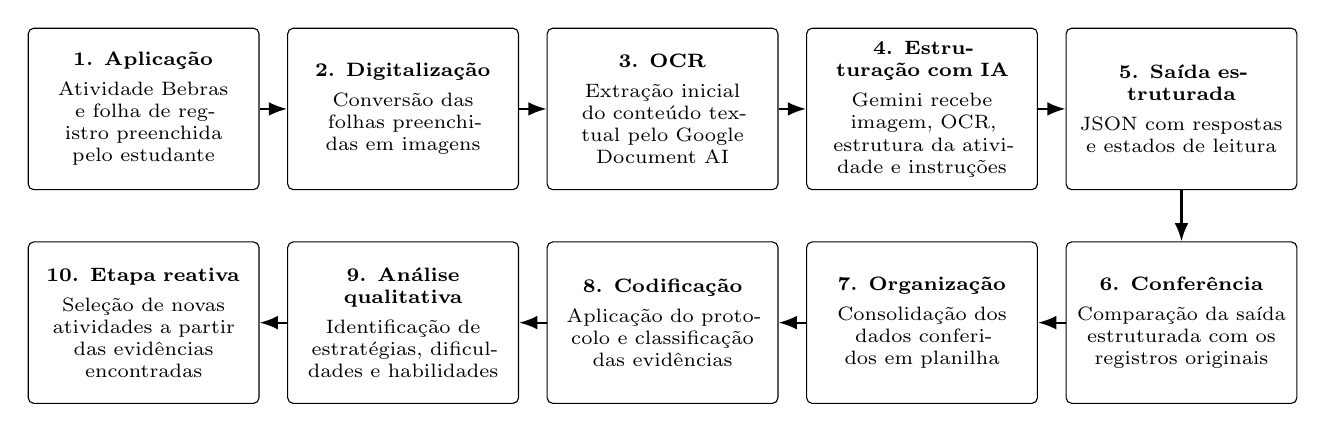
\begin{tikzpicture}[
        >=Latex,
        every node/.style={
            font=\scriptsize,
            align=center
        },
        etapa/.style={
            draw,
            rounded corners=2pt,
            text width=2.65cm,
            minimum height=2.05cm,
            inner sep=4pt
        },
        seta/.style={
            ->,
            thick
        }
    ]

    \node[etapa] (aplicacao) {
        \textbf{1. Aplicação}\\[1mm]
        Atividade Bebras e folha de registro preenchida pelo estudante
    };

    \node[etapa, right=0.35cm of aplicacao] (digitalizacao) {
        \textbf{2. Digitalização}\\[1mm]
        Conversão das folhas preenchidas em imagens
    };

    \node[etapa, right=0.35cm of digitalizacao] (ocr) {
        \textbf{3. OCR}\\[1mm]
        Extração inicial do conteúdo textual pelo Google Document AI
    };

    \node[etapa, right=0.35cm of ocr] (gemini) {
        \textbf{4. Estruturação com IA}\\[1mm]
        Gemini recebe imagem, OCR, estrutura da atividade e instruções
    };

    \node[etapa, right=0.35cm of gemini] (json) {
        \textbf{5. Saída estruturada}\\[1mm]
        JSON com respostas e estados de leitura
    };

    \node[etapa, below=0.65cm of json] (conferencia) {
        \textbf{6. Conferência}\\[1mm]
        Comparação da saída estruturada com os registros originais
    };

    \node[etapa, left=0.35cm of conferencia] (planilha) {
        \textbf{7. Organização}\\[1mm]
        Consolidação dos dados conferidos em planilha
    };

    \node[etapa, left=0.35cm of planilha] (codificacao) {
        \textbf{8. Codificação}\\[1mm]
        Aplicação do protocolo e classificação das evidências
    };

    \node[etapa, left=0.35cm of codificacao] (analise) {
        \textbf{9. Análise qualitativa}\\[1mm]
        Identificação de estratégias, dificuldades e habilidades
    };

    \node[etapa, left=0.35cm of analise] (reativa) {
        \textbf{10. Etapa reativa}\\[1mm]
        Seleção de novas atividades a partir das evidências encontradas
    };

    \draw[seta] (aplicacao) -- (digitalizacao);
    \draw[seta] (digitalizacao) -- (ocr);
    \draw[seta] (ocr) -- (gemini);
    \draw[seta] (gemini) -- (json);

    \draw[seta] (json) -- (conferencia);

    \draw[seta] (conferencia) -- (planilha);
    \draw[seta] (planilha) -- (codificacao);
    \draw[seta] (codificacao) -- (analise);
    \draw[seta] (analise) -- (reativa);

    \end{tikzpicture}

    \vspace{0.2cm}

    \begin{flushleft}
        \footnotesize
        Fonte: Elaborado pela autora (2026).
    \end{flushleft}

\end{figure}

\subsection{Aspectos éticos e preservação dos registros}

Os registros produzidos pelos estudantes são utilizados exclusivamente para os objetivos da pesquisa. A identificação dos participantes é preservada durante a organização dos dados, a análise e a apresentação dos resultados.

A realização da pesquisa no contexto escolar foi autorizada pela instituição participante, conforme Carta de Aceite apresentada no Anexo~\ref{anexo:carta-aceite}.

\section{RESULTADOS PARCIAIS E ANDAMENTO DA PESQUISA}

Até o momento, foi realizada uma análise piloto de dez registros, sendo cinco referentes à atividade As Chaves do Cofre e cinco à atividade Água para Todos. A unidade principal de análise corresponde às respostas e representações produzidas pelos estudantes em cada questão, considerando conjuntamente textos, sequências, desenhos, setas, marcações e outros elementos presentes nas folhas de registro.

As evidências foram classificadas como \textit{evidência clara}, \textit{evidência parcial} ou \textit{sem evidência suficiente}, conforme os critérios apresentados na metodologia. Essas categorias expressam a força da evidência disponível no registro analisado e não constituem notas ou níveis de domínio das habilidades. As contagens apresentadas nesta seção possuem caráter descritivo e auxiliam na identificação de tendências do conjunto piloto.

Os resultados parciais são apresentados em duas dimensões. A primeira reúne as evidências relacionadas às habilidades de Pensamento Computacional e às estratégias de resolução observadas nos registros. A segunda apresenta aspectos identificados durante a aplicação do processo de coleta, organização e análise dos dados.

\subsection{Evidências parciais sobre aprendizagem e a mobilização das estratégias de resolução}
%%deixar mais claro como foi feita a analise qualitativa 
A Tabela~\ref{tab:evidencias-piloto} apresenta uma síntese das evidências identificadas nos dez registros selecionados para a análise piloto. Foram considerados cinco registros de cada atividade. As contagens representam a ocorrência das categorias nos registros analisados, sem constituir medida de domínio das habilidades pelos estudantes.

{
\begin{table}[htbp]
    \centering

    \captionsetup{
        font=footnotesize,
        justification=raggedright,
        singlelinecheck=false
    }

    \caption{Distribuição das evidências identificadas na análise piloto}
    \label{tab:evidencias-piloto}

    \footnotesize
    \renewcommand{\arraystretch}{1.15}
    \setlength{\tabcolsep}{4pt}

    \begin{tabularx}{\textwidth}{
        >{\raggedright\arraybackslash}p{3cm}
        >{\raggedright\arraybackslash}X
        >{\centering\arraybackslash}p{1.15cm}
        >{\centering\arraybackslash}p{1.25cm}
        >{\centering\arraybackslash}p{2.15cm}
    }

        \hline

        \textbf{Atividade} &
        \textbf{Habilidade} &
        \textbf{Clara} &
        \textbf{Parcial} &
        \makecell{\textbf{Sem evidência}\\\textbf{suficiente}} \\
        \hline

        As Chaves do Cofre &
        Pensamento algorítmico &
        5 & 0 & 0 \\

        &
        Decomposição &
        0 & 1 & 4 \\

        &
        Abstração &
        0 & 2 & 3 \\

        &
        Avaliação e depuração &
        3 & 2 & 0 \\

        &
        Reconhecimento de padrões &
        0 & 0 & 5 \\
        \hline

        Água para Todos &
        Pensamento algorítmico &
        4 & 1 & 0 \\

        &
        Decomposição &
        4 & 1 & 0 \\

        &
        Abstração &
        4 & 1 & 0 \\

        &
        Avaliação e depuração &
        3 & 0 & 2 \\

        &
        Reconhecimento de padrões &
        0 & 0 & 5 \\
        \hline

    \end{tabularx}

    \vspace{1mm}

    \begin{flushleft}
        \footnotesize
        Fonte: Elaborado pela autora a partir dos registros analisados (2026).

        Nota: foram analisados cinco registros de cada atividade.
        As categorias indicam a evidência disponível no registro e não representam níveis de domínio das habilidades pelos estudantes.
    \end{flushleft}

\end{table}
}

O pensamento algorítmico foi a habilidade com evidências mais consistentes nas duas atividades. Em \textit{As Chaves do Cofre}, os cinco registros apresentaram evidência clara dessa habilidade. Em
\textit{Água para Todos}, quatro registros foram classificados com evidência clara e um com evidência parcial. Os registros analisados apresentaram, principalmente, sequências de ações e formas organizadas de representar o percurso utilizado na resolução.

A decomposição apresentou diferenças entre as duas tarefas. Em \textit{As Chaves do Cofre}, foi identificada uma evidência parcial, enquanto os demais registros não forneceram elementos suficientes para sustentar essa classificação. Em \textit{Água para Todos}, quatro registros apresentaram evidência clara e um apresentou evidência parcial. A estrutura da segunda atividade favoreceu registros em que os estudantes analisaram diferentes partes do problema e relacionaram resultados parciais para chegar à solução.

Comportamento semelhante foi observado na abstração. Na atividade As Chaves do Cofre, foram identificadas duas evidências parciais e três registros sem evidência suficiente. Em Água para Todos, quatro registros apresentaram evidência clara e um apresentou evidência parcial. Nessa tarefa, desenhos, marcações e seleção de elementos do problema contribuíram para tornar mais visíveis as formas de representação utilizadas pelos estudantes.

A avaliação e a depuração também apareceram nas duas atividades. Em As Chaves do Cofre, três registros apresentaram evidência clara e dois, evidência parcial. Em Água para Todos, foram identificadas três evidências claras e dois registros sem evidência
suficiente. Entre os elementos observados estão a comparação entre possibilidades, a verificação da resposta e o registro de alternativas que não atenderam às condições da tarefa.

O reconhecimento de padrões foi a habilidade menos evidenciada no conjunto piloto. Nenhum dos dez registros apresentou elementos suficientes para classificá-la como evidência clara ou parcial. Esse
resultado não permite concluir que os estudantes não possuam ou não tenham mobilizado essa habilidade. Ele indica que, nas produções analisadas, os registros disponíveis não permitiram identificá-la de forma sustentada.

A comparação entre as duas atividades também mostra que diferentes tarefas podem tornar determinadas habilidades mais visíveis. Enquanto As Chaves no Cofre produziu evidências mais fortes de pensamento algorítmico e avaliação, Água para Todos favoreceu a observação de decomposição, abstração e pensamento algorítmico. Dessa forma, a análise piloto reforça a necessidade de considerar um conjunto de situações-problema, pois uma única atividade não oferece as mesmas oportunidades de registro para todas as habilidades investigadas.

\subsection{Experiência adquirida através do processo de coleta e análise}

A análise piloto também permitiu avaliar o próprio processo de coleta e organização dos dados. Um dos aspectos observados foi a importância de solicitar registros adicionais à alternativa escolhida. Em diferentes casos, a resposta final fornecia pouca informação sobre o percurso de resolução, enquanto justificativas, sequências, desenhos e marcações permitiam identificar estratégias utilizadas pelo estudante.

As formas gráficas de registro mostraram-se especialmente relevantes. Setas, esquemas, marcações sobre a própria atividade e outras representações nem sempre poderiam ser adequadamente compreendidas a partir de uma transcrição textual isolada. Por essa razão, a imagem original permanece como fonte principal durante a conferência e a análise dos dados.

A aplicação do protocolo de codificação também mostrou a necessidade de distinguir a habilidade inicialmente associada à tarefa das habilidades que podem aparecer nos registros produzidos pelos estudantes. A classificação prevista para cada atividade orienta a coleta, porém não limita a análise. Quando uma produção apresenta elementos compatíveis com outra habilidade, esses elementos também podem ser considerados, desde que sustentados pelos critérios definidos no protocolo.

O processo de digitalização e estruturação automática também apresentou limitações. O reconhecimento de texto manuscrito pode ser afetado por rasuras, setas, desenhos, escrita sobre imagens e outras formas de registro. A etapa com o modelo generativo auxilia na organização das informações em uma estrutura padronizada, mas a conferência com as folhas originais continua necessária antes da utilização dos dados na análise qualitativa.

A aplicação do protocolo de codificação também mostrou a necessidade de distinguir a habilidade inicialmente associada à tarefa das habilidades que podem aparecer nos registros produzidos pelos estudantes. A classificação prevista para cada atividade orienta a coleta, porém não limita a análise. Quando uma produção apresenta elementos compatíveis com outra habilidade, esses elementos também podem ser considerados, desde que sustentados pelos critérios definidos no protocolo.

A utilização das categorias evidência clara, evidência parcial e sem evidência suficiente contribuiu para explicitar os limites da interpretação. Em alguns registros havia indícios de determinada estratégia, mas a explicação produzida pelo estudante não era suficiente para uma classificação mais forte. A categoria sem evidência suficiente mostrou-se particularmente importante para evitar que a ausência de informações no registro fosse interpretada como ausência da habilidade.

A organização e a conferência dos registros também mostraram-se etapas trabalhosas. Cada folha precisa ser examinada considerando textos manuscritos, marcações, desenhos, setas, rasuras e respostas distribuídas em diferentes partes do documento. Mesmo com o apoio do OCR e da estruturação automática, a comparação com a imagem original continua necessária, principalmente quando a escrita é pouco legível ou quando a informação relevante está representada de forma gráfica. A realização integral desse processo de forma manual exigiria a transcrição e a verificação individual de cada campo, aumentando significativamente o tempo necessário para preparar o material para análise e tornando mais difícil manter a padronização em um conjunto maior de registros.

Essa dificuldade é ampliada pela própria diversidade das produções dos estudantes. Nem todos respondem às folhas com o mesmo nível de detalhamento. Alguns registram sequências, justificativas, tentativas e formas de verificação, enquanto outros indicam apenas a alternativa final, deixam campos em branco ou produzem respostas muito breves. Dessa forma, a quantidade e a qualidade das evidências disponíveis dependem também do envolvimento do estudante com a proposta de explicitar seu processo de resolução.

A ausência de evidência suficiente pode, portanto, ter diferentes origens. O estudante pode não ter mobilizado determinada habilidade durante a resolução; pode tê-la mobilizado, mas não a ter registrado de forma suficientemente clara; ou pode ter produzido um registro limitado por baixa participação na atividade. Também é possível que a tarefa seja resolvida por uma estratégia diferente daquela prevista no planejamento, sem tornar observável a habilidade inicialmente associada ao problema.

Essas situações afetam tanto a etapa de conferência quanto a interpretação dos resultados. Registros mais completos oferecem mais elementos para a codificação, enquanto produções reduzidas aumentam a incerteza e podem exigir maior retorno à folha original. Por esse motivo, a categoria sem evidência suficiente indica apenas que o material disponível não permite sustentar a identificação da habilidade naquele registro. Ela não permite concluir, de forma isolada, que o estudante não possui a habilidade ou que apresentou dificuldade para mobilizá-la.

As contagens apresentadas nos resultados devem, assim, ser interpretadas como uma descrição das evidências disponíveis nas produções coletadas. Diferenças na participação dos estudantes, na forma de registrar o raciocínio e nas estratégias escolhidas podem influenciar a distribuição das categorias observadas. Por isso, esses valores não constituem uma medida direta da presença, ausência ou domínio das habilidades de Pensamento Computacional.

Por fim, os códigos utilizados na análise inicial identificam os registros de cada atividade e não permitem estabelecer uma comparação linear entre os mesmos estudantes nas diferentes tarefas. As interpretações apresentadas, portanto, referem-se ao conjunto de produções analisadas em cada atividade.

\subsection{Próximas etapas}

A continuidade da pesquisa envolve a ampliação da codificação para os demais registros coletados e a aplicação do protocolo refinado ao conjunto completo de dados. A análise piloto será utilizada como referência para verificar a consistência dos critérios e realizar ajustes quando surgirem situações ainda não contempladas. 

A etapa diagnóstica reativa considerará principalmente as habilidades que permaneceram pouco evidenciadas nas aplicações anteriores. O reconhecimento de padrões constitui, neste momento, um dos focos prioritários, enquanto decomposição e abstração poderão ser novamente observadas em tarefas com características distintas das já aplicadas.

Com a ampliação do conjunto analisado, será possível examinar recorrências nas estratégias utilizadas, dificuldades encontradas, formas de representação e procedimentos de verificação. A análise final também deverá discutir as contribuições e limitações do processo computacional utilizado para organizar os registros, especialmente nos casos que exigem revisão humana devido a escrita manuscrita, símbolos, desenhos ou outras formas de representação.

\section{Considerações Parciais}



%\section{Apenas na entrega final para defesa: Conclusão}

%Esta seção deve fazer uma síntese do trabalho (é quase um resumo do passado), as principais contribuições (o que foi entregue), uma discussão da avaliação (o que deu certo e quais as limitações) e os possíveis trabalhos futuros.

%Aqui também vale relembrar onde o software está disponível, repositório de código, etc.



% ----------------------------------------------------------
% ELEMENTOS PÓS-TEXTUAIS
% ----------------------------------------------------------
\newpage
\postextual

% ----------------------------------------------------------
% Referências bibliográficas
% ----------------------------------------------------------
\bibliography{references}

% ----------------------------------------------------------
% Glossário
% ----------------------------------------------------------
%
% Há diversas soluções prontas para glossário em LaTeX. 
% Consulte o manual do abnTeX2 para obter sugestões.
%
%\glossary

% ----------------------------------------------------------
% Apêndices
% ----------------------------------------------------------

\newpage
\appendix
\begin{apendicesenv}
\section{Folha de registro da atividade As Chaves do Cofre}
\label{apendice:chaves-cofre}

A folha de registro apresentada a seguir foi elaborada para coletar
informações sobre o processo de resolução da atividade
\textit{As Chaves do Cofre}.

\section{Folha de registro da atividade Água para Todos}
\label{apendice:agua-todos}

A folha de registro apresentada a seguir foi elaborada para coletar
informações sobre o processo de resolução da atividade
\textit{Água para Todos}.

\section{Prompt utilizado na estruturação dos registros com Gemini}
\label{apendice:prompt-gemini}

O processamento dos registros utiliza instruções distintas conforme a estrutura de cada atividade. Além das imagens digitalizadas, o Gemini recebe o texto previamente extraído pelo Google Document AI e uma
descrição dos campos presentes na atividade.

Na atividade \textit{As Chaves do Cofre}, o processamento utiliza uma única imagem, correspondente à folha preenchida pelo estudante. Na atividade \textit{Água para Todos}, são utilizadas duas imagens: a folha da questão, que pode conter marcações realizadas diretamente
sobre o mapa, e a folha de registro.

A resposta do modelo é solicitada em formato JSON e segue uma estrutura previamente definida pelo programa para cada atividade. Os prompts utilizados são apresentados nas subseções seguintes.


\subsection*{Prompt para a atividade As Chaves do Cofre}

Na atividade \textit{As Chaves do Cofre}, o Gemini recebe a imagem JPG da folha preenchida pelo estudante, o texto extraído pelo OCR e a descrição da estrutura da atividade.

O prompt utilizado é apresentado a seguir. Os elementos entre chaves são substituídos automaticamente pelo programa durante o processamento.

\begin{lstlisting}[style=prompt]
Você está analisando uma folha de registro de um estudante
na atividade Bebras:

"{configuracao['nome']}"

A imagem contém elementos impressos da atividade
e respostas produzidas pelo estudante.

As respostas podem conter:

- texto manuscrito;
- alternativas marcadas;
- desenhos;
- setas;
- formas geométricas;
- sequências;
- riscos;
- outras representações.

O texto abaixo foi extraído pelo Google Document AI.

--- INÍCIO DO OCR ---

{texto_ocr}

--- FIM DO OCR ---

ESTRUTURA DA ATIVIDADE:

{configuracao["descricao"]}

REGRAS:

- Use a imagem como principal fonte.
- Use o OCR somente como apoio.
- Diferencie elementos impressos das respostas do estudante.
- Não invente informações.
- Não determine a resposta correta da atividade.
- Não avalie o desempenho do estudante.
- Não atribua habilidades de Pensamento Computacional.

IMPORTANTE SOBRE DESENHOS E MARCAÇÕES:

- Descreva apenas aquilo que é diretamente visível.
- Não atribua intenção ao estudante.
- Não explique por que o estudante fez determinada marcação,
  a menos que isso esteja explicitamente escrito por ele.
- Não transforme uma marcação visual em uma conclusão
  sobre o raciocínio do estudante.
- Não use expressões como "para verificar",
  "com o objetivo de", "indicando que" ou semelhantes
  para explicar a intenção do estudante,
  a menos que essas palavras tenham sido escritas
  pelo próprio estudante.

Exemplo:

CORRETO:

"Ponto 4 circulado. Há linhas traçadas entre o ponto 4
e outros nós."

INCORRETO:

"O estudante circulou o ponto 4 para verificar se todas
as vilas estavam a duas estradas."

STATUS DAS QUESTÕES:

Use "ok" SOMENTE quando a informação estiver
diretamente legível ou visualmente identificável
sem necessidade de interpretação incerta.

Use "revisar" quando:

- alguma parte estiver ambígua;
- existir mais de uma interpretação possível;
- uma forma ou símbolo não puder ser identificado
  com total segurança;
- apenas parte de uma sequência estiver clara;
- você sentir necessidade de usar palavras como
  "parece", "possivelmente", "provavelmente",
  "aparentemente" ou "talvez".

Se houver dúvida, prefira "revisar" em vez de "ok".

Use "ilegivel" quando houver conteúdo produzido
pelo estudante, mas não for possível interpretá-lo.

Uma resposta realmente em branco deve ser null.
Uma resposta em branco pode ter status "ok",
pois foi possível verificar que o campo está vazio.

NOME DO ESTUDANTE:

- Se estiver claramente legível:
  nome_status = "ok".

- Se houver uma leitura provável, mas com dúvida:
  registre a leitura provável e use
  nome_status = "revisar".

- Se houver um nome escrito mas não for possível lê-lo:
  nome_estudante = null e
  nome_status = "ilegivel".

- Se o campo estiver vazio:
  nome_estudante = null e
  nome_status = "ausente".

Preserve o sentido original das respostas.

Corrija erros do OCR somente quando a imagem
permitir confirmar claramente o conteúdo.

Retorne somente JSON.
\end{lstlisting}


\subsection*{Estrutura informada para As Chaves do Cofre}

Além do prompt, o programa fornece ao modelo uma descrição dos campos presentes na folha de registro:

\begin{lstlisting}[
    breaklines=true,
    basicstyle=\ttfamily\scriptsize,
    columns=fullflexible,
    keepspaces=true
]
1. Qual alternativa você escolheu?
Opções: A, B, C ou D.

2. Registre a sequência de objetos utilizada.
Pode conter desenhos, formas geométricas e setas.

3. Explique como você encontrou esse caminho.
Pode conter texto, desenhos, setas ou estar em branco.

4. Você testou algum caminho que não funcionou?
Opções: Sim ou Não.
Pode existir uma representação desenhada.

5. Como você verificou que esse era o menor número
possível de gavetas?
Resposta aberta.

6. Qual foi a parte mais difícil da atividade?
Resposta aberta.

7. Depois de conversar com um colega, você mudou
sua resposta ou estratégia?
Opções: Sim ou Não.
Pode conter justificativa.
\end{lstlisting}


\subsection*{Prompt para a atividade Água para Todos}

Na atividade \textit{Água para Todos}, o Gemini recebe duas imagens do mesmo estudante. A primeira corresponde à folha da questão e do mapa, enquanto a segunda corresponde à folha de registro. O texto extraído pelo Google Document AI é obtido da folha de registro e utilizado como apoio à leitura das imagens.

O prompt utilizado é apresentado a seguir.

\begin{lstlisting}[
    breaklines=true,
    basicstyle=\ttfamily\scriptsize,
    columns=fullflexible,
    keepspaces=true
]
Você está analisando o registro de um estudante
na atividade Bebras:

"{configuracao['nome']}"

Você recebeu DUAS imagens do mesmo estudante.

IMAGEM 1:

É a folha da questão/mapa.

Ela contém elementos originalmente impressos,
mas também pode conter anotações feitas pelo estudante,
como:

- caminhos;
- setas;
- riscos;
- círculos;
- números;
- símbolos;
- marcações;
- pequenas anotações.

Essas anotações fazem parte do processo
de resolução do estudante.

IMAGEM 2:

É a folha de registro/resposta.

O texto abaixo foi extraído pelo
Google Document AI da folha de resposta.

REGRAS:

- Use a imagem como principal fonte.
- Use o OCR somente como apoio.
- Diferencie elementos impressos das respostas do estudante.
- Não invente informações.
- Não determine a resposta correta da atividade.
- Não avalie o desempenho do estudante.
- Não atribua habilidades de Pensamento Computacional.

IMPORTANTE SOBRE DESENHOS E MARCAÇÕES:

- Descreva apenas aquilo que é diretamente visível.
- Não atribua intenção ao estudante.
- Não explique por que o estudante fez determinada marcação,
  a menos que isso esteja explicitamente escrito por ele.
- Não transforme uma marcação visual em uma conclusão
  sobre o raciocínio do estudante.
- Não use expressões como "para verificar",
  "com o objetivo de", "indicando que" ou semelhantes
  para explicar a intenção do estudante,
  a menos que essas palavras tenham sido escritas
  pelo próprio estudante.

Exemplo:

CORRETO:

"Ponto 4 circulado. Há linhas traçadas entre o ponto 4
e outros nós."

INCORRETO:

"O estudante circulou o ponto 4 para verificar se todas
as vilas estavam a duas estradas."

STATUS DAS QUESTÕES:

Use "ok" SOMENTE quando a informação estiver
diretamente legível ou visualmente identificável
sem necessidade de interpretação incerta.

Use "revisar" quando:

- alguma parte estiver ambígua;
- existir mais de uma interpretação possível;
- uma forma ou símbolo não puder ser identificado
  com total segurança;
- apenas parte de uma sequência estiver clara;
- você sentir necessidade de usar palavras como
  "parece", "possivelmente", "provavelmente",
  "aparentemente" ou "talvez".

Se houver dúvida, prefira "revisar" em vez de "ok".

Use "ilegivel" quando houver conteúdo produzido
pelo estudante, mas não for possível interpretá-lo.

Uma resposta realmente em branco deve ser null.
Uma resposta em branco pode ter status "ok",
pois foi possível verificar que o campo está vazio.

NOME DO ESTUDANTE:

- Se estiver claramente legível:
  nome_status = "ok".

- Se houver uma leitura provável, mas com dúvida:
  registre a leitura provável e use
  nome_status = "revisar".

- Se houver um nome escrito mas não for possível lê-lo:
  nome_estudante = null e
  nome_status = "ilegivel".

- Se o campo estiver vazio:
  nome_estudante = null e
  nome_status = "ausente".

Preserve o sentido original das respostas.

Corrija erros do OCR somente quando a imagem
permitir confirmar claramente o conteúdo.

Retorne somente JSON.

--- INÍCIO DO OCR ---

{texto_ocr}

--- FIM DO OCR ---

ESTRUTURA DA ATIVIDADE:

{configuracao["descricao"]}

REGRAS:

- Analise as duas imagens em conjunto.
- Use as imagens como principal fonte.
- Use o OCR somente como apoio textual.
- Considere as anotações feitas na folha da questão.
- Diferencie elementos impressos dos elementos
  acrescentados pelo estudante.
- Não invente informações.
- Não determine a resposta correta.
- Não avalie o estudante.
- Não atribua habilidades de Pensamento Computacional.
- Apenas transcreva e descreva aquilo que foi registrado.
- Preserve o sentido original das respostas.
- Uma resposta realmente em branco deve ser null.
- Não confunda resposta em branco com conteúdo ilegível.
- Se houver ambiguidade, use status "revisar".
- Se houver conteúdo ilegível, use status "ilegivel".
- Se estiver claro, use status "ok".
- Se um campo não puder ser determinado com segurança,
  retorne null e continue preenchendo os demais.

Retorne somente JSON.
\end{lstlisting}


\subsection*{Estrutura informada para Água para Todos}

A descrição da folha de registro fornecida ao modelo é a seguinte:

\begin{lstlisting}[
    breaklines=true,
    basicstyle=\ttfamily\scriptsize,
    columns=fullflexible,
    keepspaces=true
]
1. Qual alternativa você escolheu?
Opções: A, B, C ou D.

2. Mostre como você analisou os caminhos do mapa
para chegar à resposta.
Pode conter desenhos, marcações, setas, texto ou símbolos.

3. Quais pontos você chegou a considerar antes
de escolher a resposta final?
Podem ser marcados os pontos 1, 2, 3 e 4.
Também pode ser marcada a opção indicando que
apenas a resposta final foi considerada.

4. Você testou algum ponto que não funcionou?
Opções: Sim ou Não.
Pode haver explicação ou representação do ponto testado.

5. Como você verificou que, com o ponto escolhido,
todas as vilas ficam a no máximo duas estradas
de um centro de distribuição?
Pode conter texto, desenhos ou marcações.

6. Qual foi a parte mais difícil da atividade?
Resposta aberta.

7. Depois de conversar com um colega, você mudou
sua resposta ou estratégia?
Opções: Sim ou Não.
Pode conter justificativa.
\end{lstlisting}


\subsection*{Estrutura da saída}

A saída do Gemini é restringida por um esquema JSON definido
previamente para cada atividade. O esquema determina os campos que
podem ser retornados e seus respectivos tipos de dados.

Em ambas as atividades, a estrutura contém a identificação da
atividade, o nome do estudante, o estado de leitura do nome, o ano e
os campos correspondentes às sete questões da folha de registro.

O campo \texttt{nome\_status} pode assumir os valores
\texttt{ok}, \texttt{revisar}, \texttt{ilegivel} ou
\texttt{ausente}. Para as questões, são utilizados os estados
\texttt{ok}, \texttt{revisar} e \texttt{ilegivel}.

O valor \texttt{null} pode ser utilizado quando um campo está em branco
ou quando determinada informação não pode ser preenchida com segurança,
conforme as regras estabelecidas no prompt. Os campos específicos
dependem do tipo de questão e podem armazenar alternativas, textos,
listas, valores booleanos ou descrições de representações produzidas
pelo estudante.

O programa solicita ao modelo uma resposta com o tipo
\texttt{application/json} e utiliza o esquema correspondente à
atividade para restringir a estrutura retornada. Após o processamento,
o JSON é normalizado e seus dados são utilizados para gerar a planilha
empregada na etapa de conferência.
\end{apendicesenv}



% ----------------------------------------------------------
% Anexos
% ----------------------------------------------------------
%\cftinserthook{toc}{AAA}
% ---
% Inicia os anexos
% ---
%\anexos
\begin{anexosenv}
\partanexos

\chapter{Carta de Aceite da instituição participante}
\label{anexo:carta-aceite}

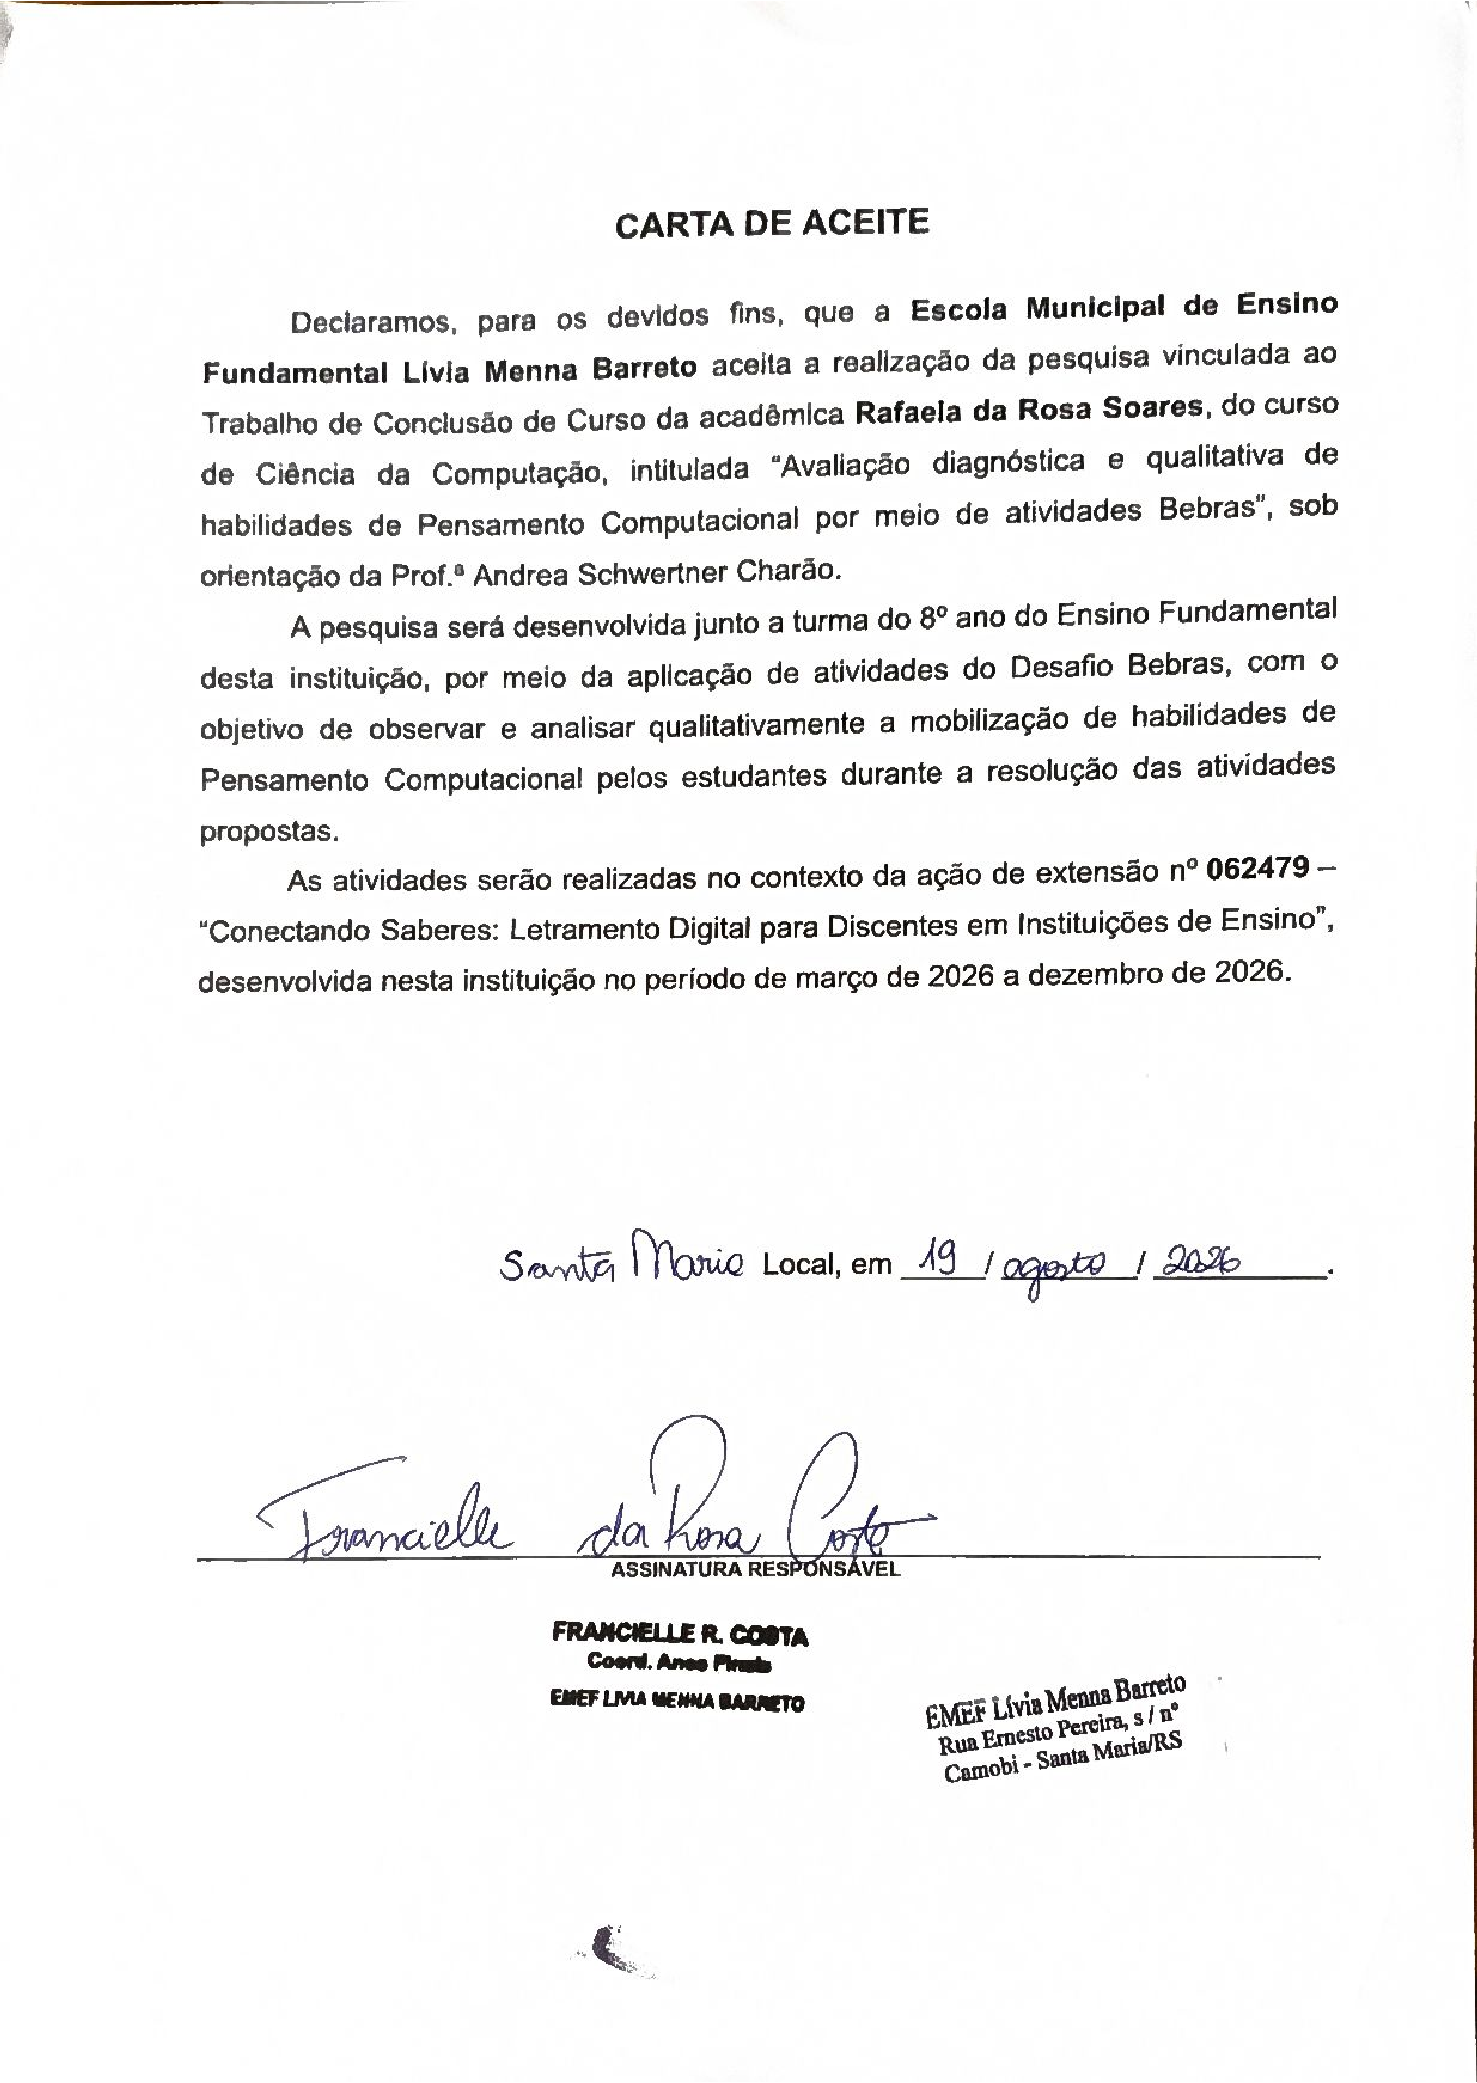
\includepdf[
    pages=-,
    pagecommand={}
]{anexos/carta_aceite.pdf}

\chapter{Folha-registro da atividade As Chaves do Cofre}
\label{anexo:chaves-do-cofre}

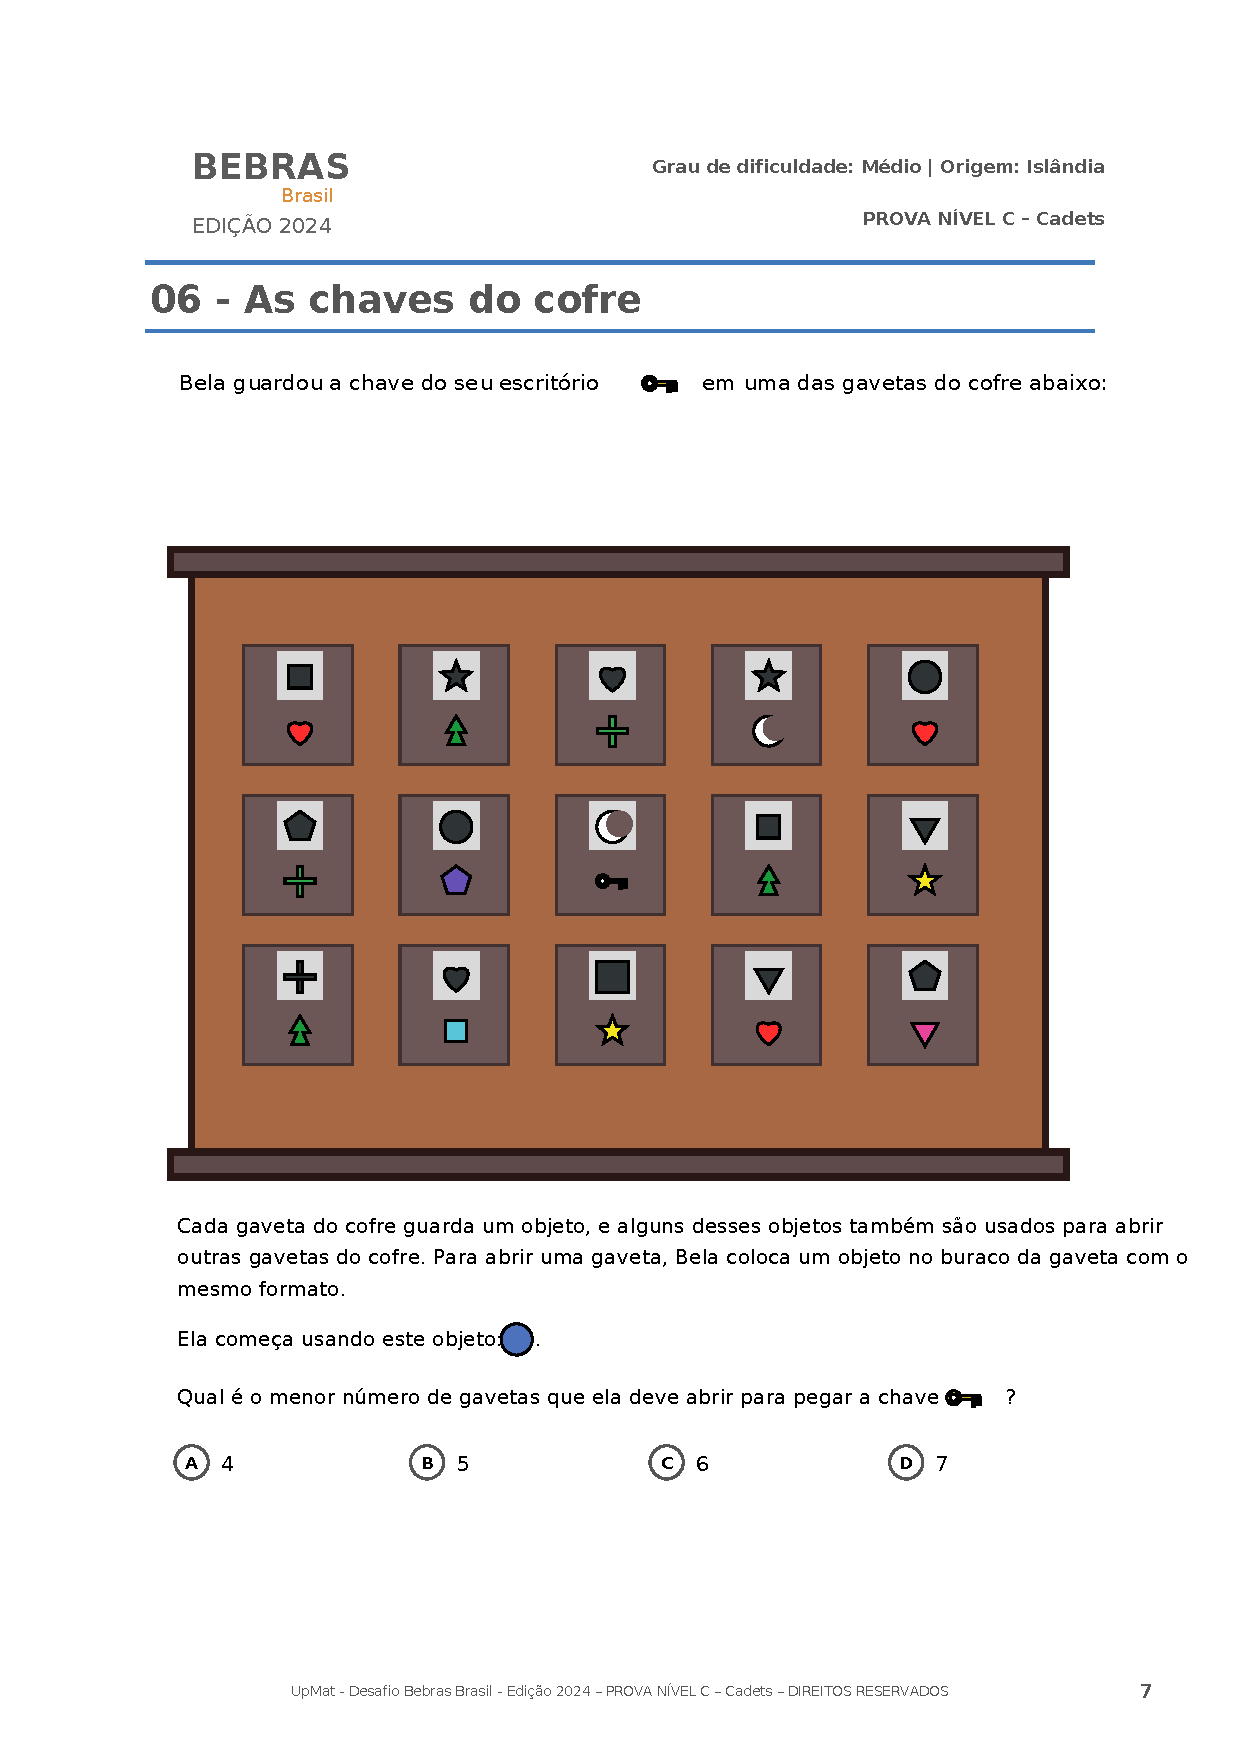
\includepdf[
    pages=-,
    pagecommand={}
]{anexos/As_Chaves_do_Cofre.pdf}

\chapter{Folha-registro da atividade Água Para Todos}
\label{anexo:agua-para-todos}

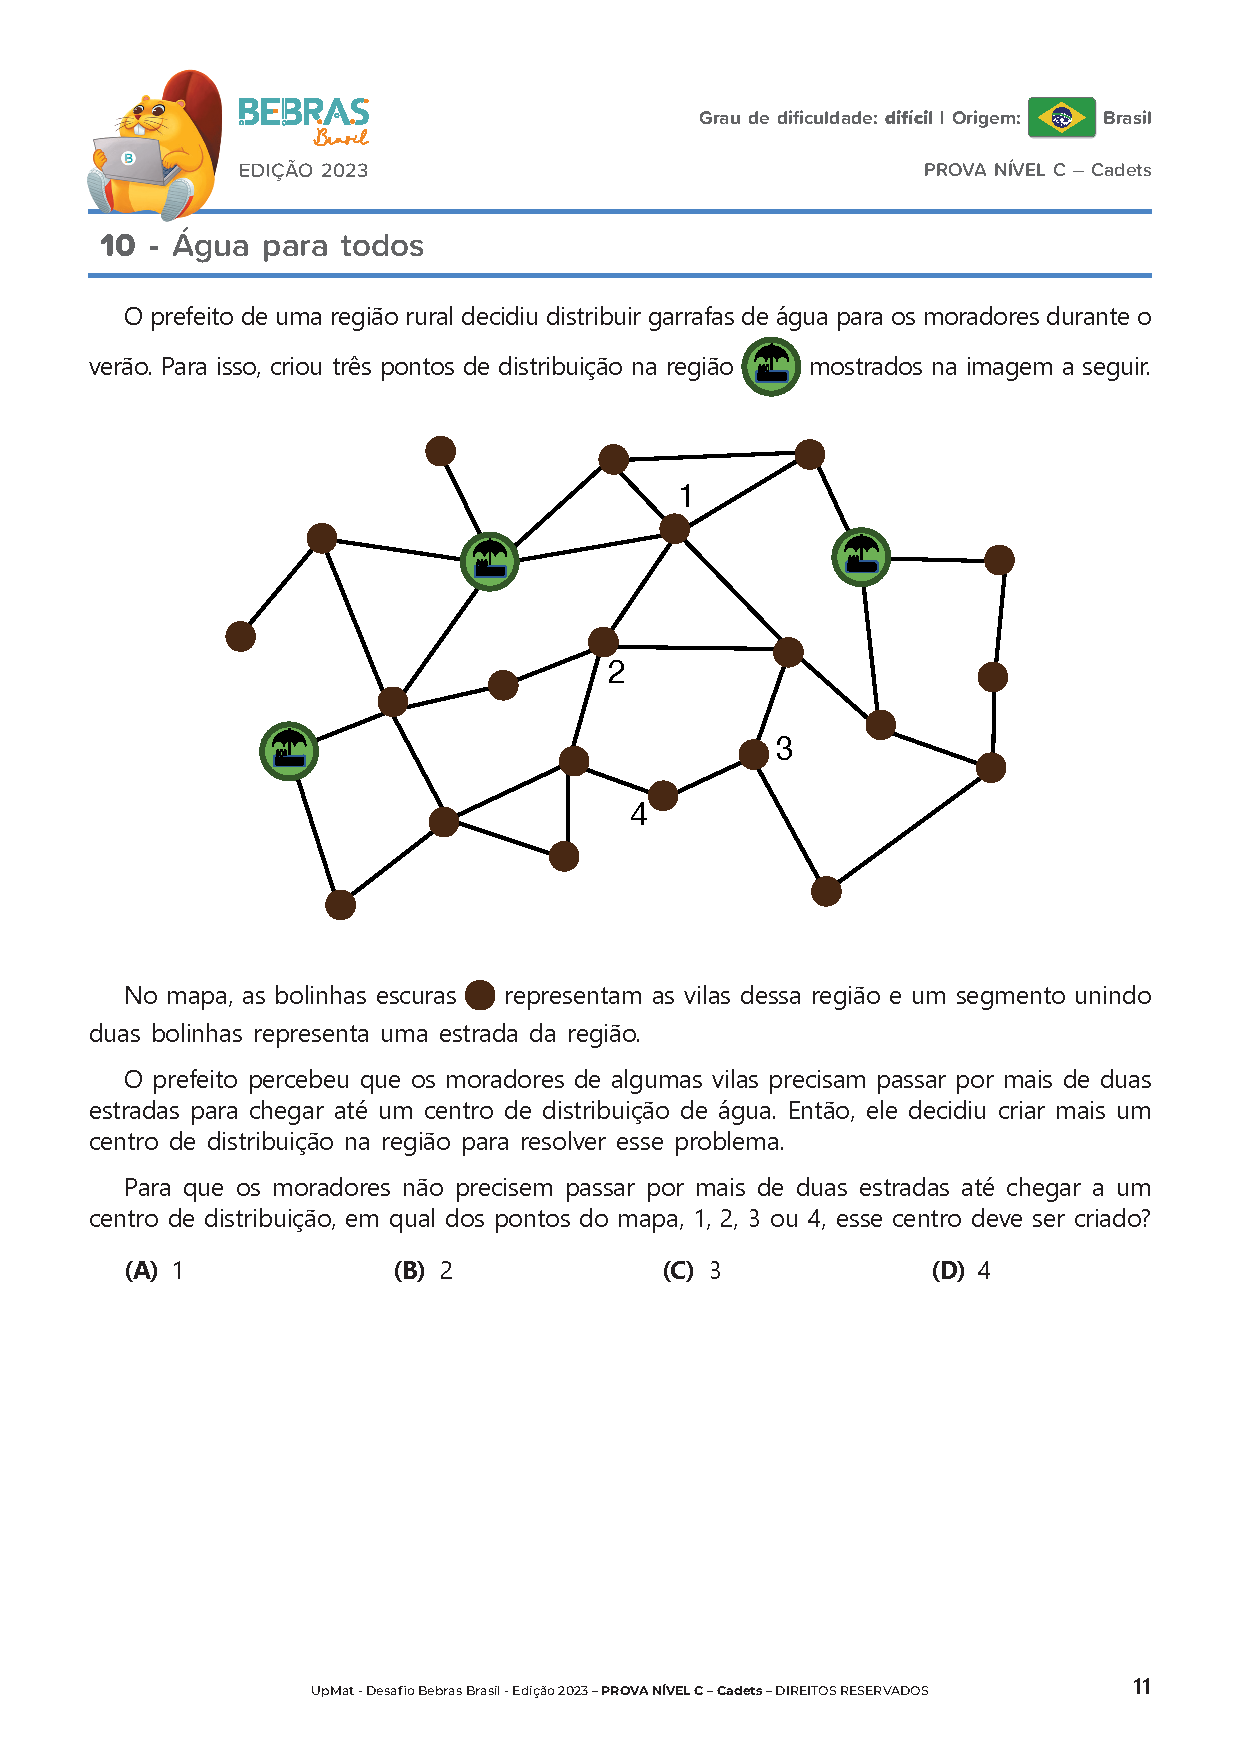
\includepdf[
    pages=-,
    pagecommand={}
]{anexos/Agua_para_Todos.pdf}

\end{anexosenv}
\end{document}

